\chapter{Wide field image synthesis}
In this chapter we discuss how the Radio Interferometric Measurement Equation can be inverted to obtain a synthesized image of the radio sky. First an overview of the imaging pipeline is given, before
delving into the finer details of creating what is known as ``dirty'' images of the sky and correcting the wide field distortions introduced in the images when breaking the assumptions made when the images 
are synthesized using a Fast Fourier Transform. Finally we discuss previous literature on acceleration of the correcting process, before moving onto the design of our imager in the following chapter. Before
continuing readers not familiar with Fourier theory should refer to Appendix~\ref{chp_DSP} for a refresher on basic signal processing concepts.
\section{The calibration, imaging and deconvolution pipeline}
The RIME can be thought of as the equation that predicts what measurement the telescope should make, given a model radio sky (\emph{intensity distribution}), telescope behavior and environmental effects as inputs. 
If all the information is known the inversion of this equation is as simple as taking an inverse Fourier Transform. To see why this is true consider that the continuous sky is simply an infinite sequence of 
shifted and scaled impulses (or delta functions), where each impulse is infinitesimally narrow, has an area of 1 and is infinitely high at the shifted position (zero everywhere else). The Fourier transform 
of each of the delta functions is simply:
\begin{equation}
 \label{eqn_delta_response}
 h(u,v) := \int_{-\infty}^\infty\int_{-\infty}^\infty \delta(l-l_0,m-m_0)e^{-2\pi i(u(l-l_0)+v(m-m_0))}dldm
\end{equation}
Observe that this is practically the same as the RIME. If the delta functions are replaced with the scaled intensities over infinitesimally small areas of the sky as defined previously and the direction dependent and
independent terms are added in the convolution integral the two integrals are practically identical, apart from the $w(\sqrt{1-l^2-m^2}-1)$ term in the complex exponent and the $n = \sqrt{1-l^2-m^2}$ in the denumerator. 
For narrow fields of view these terms are negligible. We will revisit this assumption later on when discussing the wide field problem.

In order to get the \emph{observed} intensity distribution back the Fourier transform can simply be inverted. However, inversion is not all the synthesis imaging problem entails; a distinction has to be drawn
between the \emph{observed} and \emph{true} radio sky: how much of the \emph{true} radio sky can be recovered, given the imperfect measurements made with a radio interferometer over a limited amount of time? Foremost, the
effects of limited sampling in the measurement/Fourier space (uv plane) must be considered. Formally the tracks depicted in Figure~\ref{fig_evla_observation} is called the sampling function and is defined as being 1 wherever 
a measurement is made and 0 everywhere else. The observed measurements (\emph{visibilities}) are therefore a multiplication with this sampling function, $S(u,v)$:
\begin{equation}
 V_{\text{obs}}(u,v) := V_{\text{RIME}}(u,v)S(u,v)
 \label{eqn_observed_vis}
\end{equation}

When equation~\ref{eqn_observed_vis} is inverted the extent of the problem becomes apparent:
\begin{equation}
 B_{\text{obs}}(l,m) = (G_p(t,\nu)D_p(l,m,t,\nu)I_{\text{true}}(l,m)D_q^H(l,m,t,\nu)G_q^H(t,\nu))*\psf{(l,m,\nu)} + \eta
\end{equation}
where the G terms are the directional independent gains, the D terms are the directional dependent gains and the Point Spread Function, $\psf$, is the Fourier Transform of the sampling function, $S$. Since
the u,v coordinates depend on the wavelength the $\psf$ in turn also scales depending on wavelength. $\eta$ represents the background noise level that depends on system temperature, integration time and integration
bandwidth as mentioned previously.

Not all the information we need to accurately reconstruct the true intensity distribution, $I_{\text{true}}$, is available. In fact the $\psf$ alone provides a challenging
problem by itself. The more complete the sampling function, the more accurately the image can be reconstructed. If measurements are taken over too short an observation there is
no hope of deconvolving most of the $\psf$ from the image. Even more concerning is the fact that the directional dependent effects cause a time-dependent convolution with the
true measurements and serve to modulate different parts of the synthesized image at different levels during the course of an observation. Figure~\ref{fig_psf} shows how the 
$\psf$ gradually improves with longer observation time, while Figure~\ref{fig_model_convolution} provides a good illustration of the challenge astronomers face 
when just considering the effects of limited sampling on the true sky, let alone telescope sensitivity and the direction dependent and independent effects.
\begin{figure}[h]
 \begin{mdframed}
 \centering
 \begin{subfigure}[b]{0.24\textwidth}
  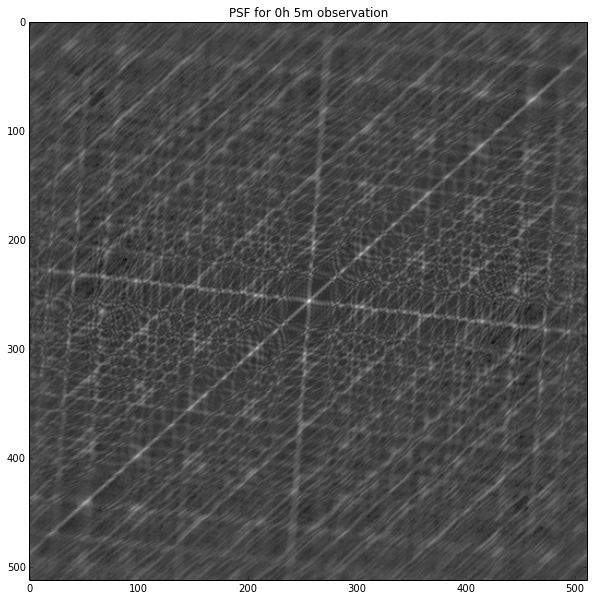
\includegraphics[width=\textwidth]{images/evla_observation_psf/5min.png}
  \caption{5 min snapshot}
 \end{subfigure}
 \begin{subfigure}[b]{0.24\textwidth}
  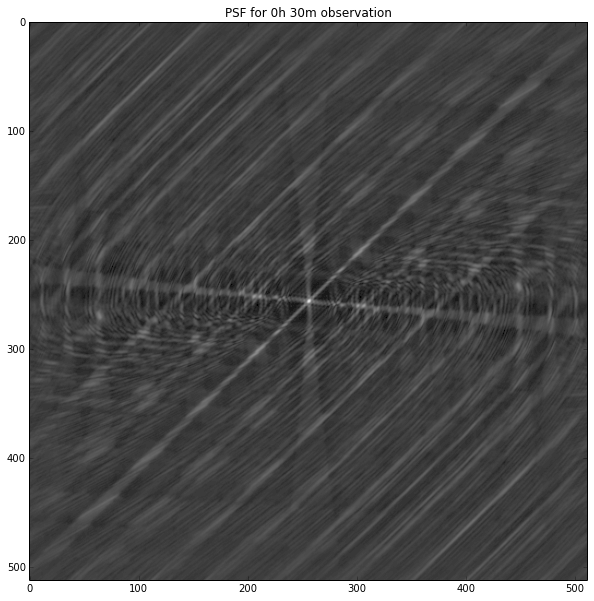
\includegraphics[width=\textwidth]{images/evla_observation_psf/30min.png}
  \caption{30 min}
 \end{subfigure}
 \begin{subfigure}[b]{0.24\textwidth}
  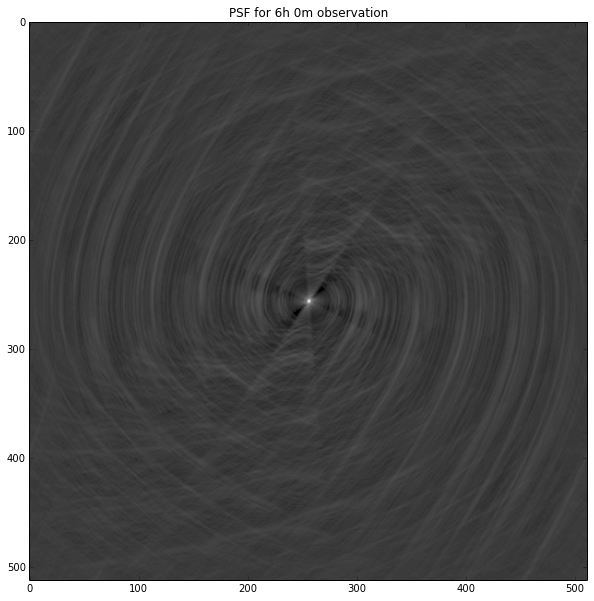
\includegraphics[width=\textwidth]{images/evla_observation_psf/6hr.png}
  \caption{6 hrs}
 \end{subfigure}
 \begin{subfigure}[b]{0.24\textwidth}
  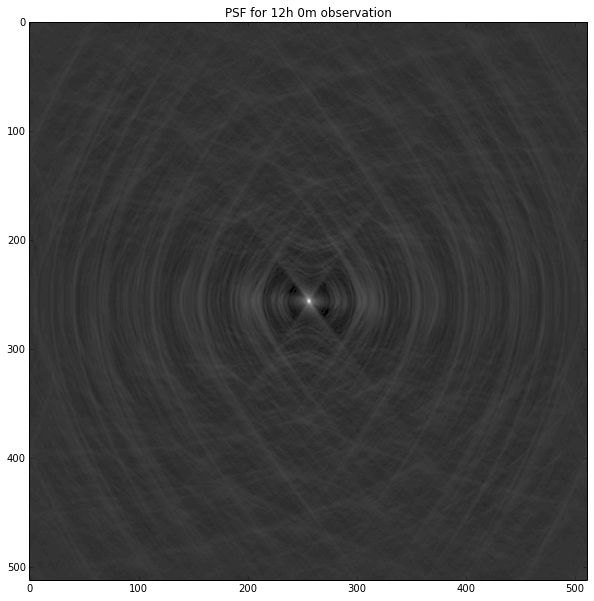
\includegraphics[width=\textwidth]{images/evla_observation_psf/12hr.png}
  \caption{12 hrs}
 \end{subfigure}
 \caption[EVLA Point Spread Function evolution]{Here the Point Spread Function is shown for various observation lengths on the EVLA D-configuration at $\delta=30^\circ$. The PSF gradually 
 becomes more defined with longer observation time. Removing the repeating lobe-like structure around the source (clearly visible in the longer observations) is the primary goal of 
 deconvolution, since it both suppresses fainter sources and adds structure and amplification to the background noise in the image.}
  \label{fig_psf}
 \end{mdframed}
\end{figure}

\begin{figure}[ht!]
 \begin{mdframed}
 \centering
 \begin{subfigure}[b]{0.39\textwidth}
  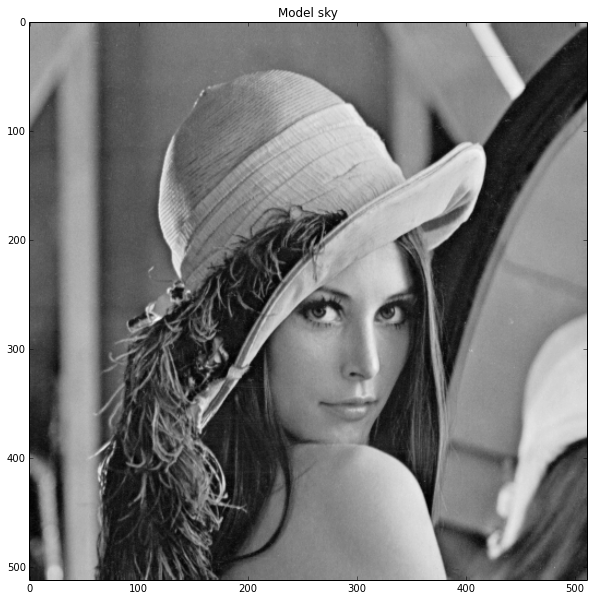
\includegraphics[width=\textwidth]{images/evla_lena_observation/model.png}
  \caption{``True''/model sky}
 \end{subfigure}
 \begin{subfigure}[b]{0.39\textwidth}
  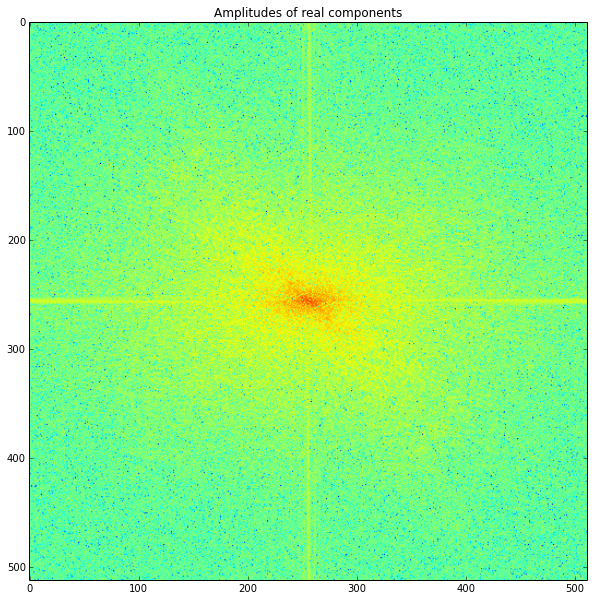
\includegraphics[width=\textwidth]{images/evla_lena_observation/real_FT.png}
  \caption{Real component of measurement/fourier space, shifted so that the DC component is at the centre pixel.}
 \end{subfigure}
 \begin{subfigure}[b]{0.34\textwidth}
  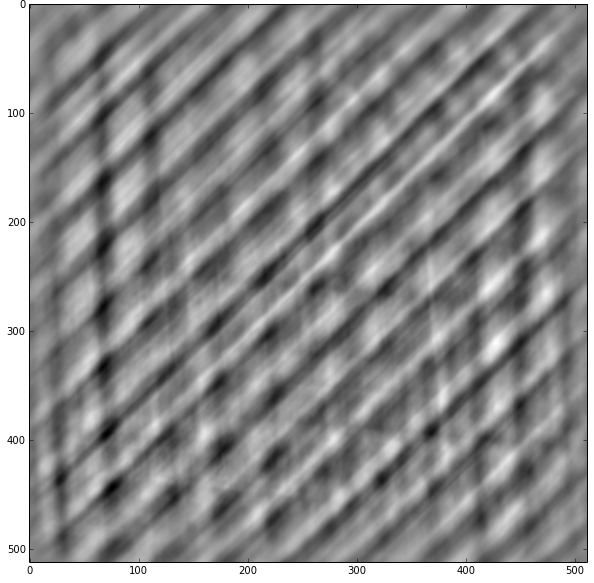
\includegraphics[width=\textwidth]{images/evla_lena_observation/30min.png}
  \caption{Dirty image after 30 min}
 \end{subfigure}
 \begin{subfigure}[b]{0.34\textwidth}
  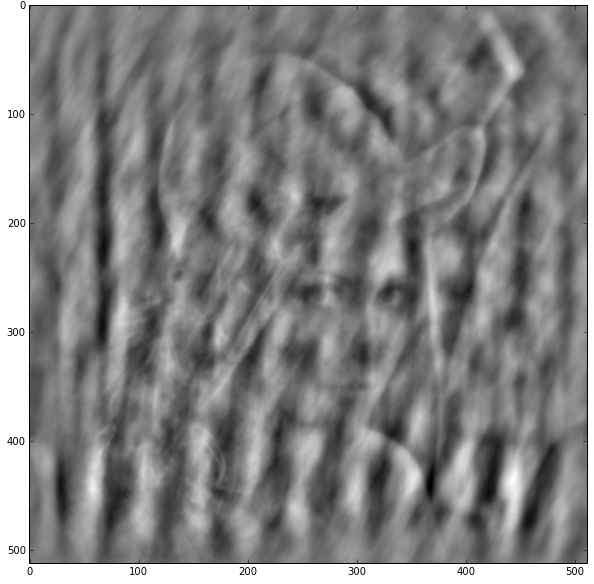
\includegraphics[width=\textwidth]{images/evla_lena_observation/6hr.png}
  \caption{Dirty image after 6 hrs}
 \end{subfigure}
 \begin{subfigure}[b]{0.34\textwidth}
  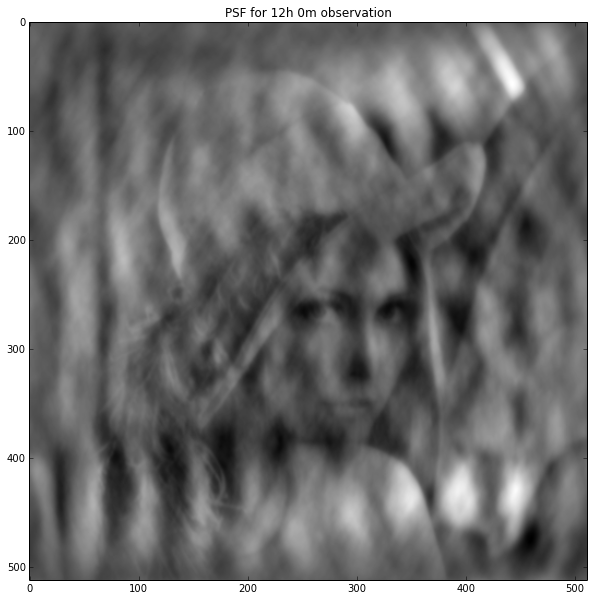
\includegraphics[width=\textwidth]{images/evla_lena_observation/12hr.png}
  \caption{Dirty image after 12 hrs}
 \end{subfigure}
 \begin{subfigure}[b]{0.34\textwidth}
  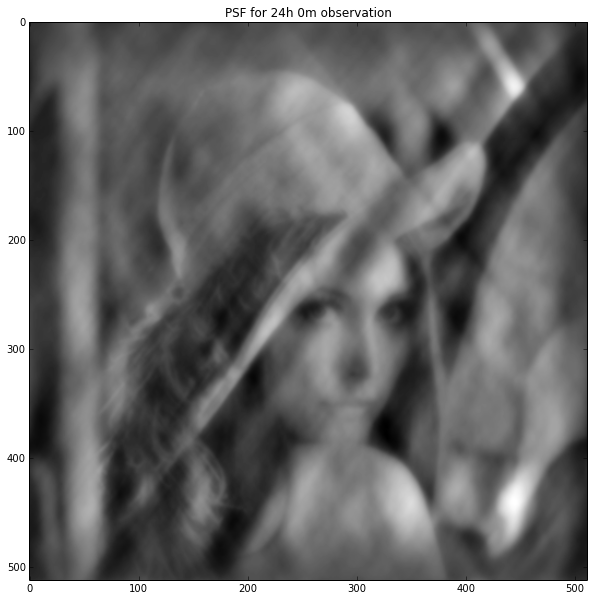
\includegraphics[width=\textwidth]{images/evla_lena_observation/24hr.png}
  \caption{Dirty image after 24 hrs}
 \end{subfigure}
 \caption[Effect of observation time on dirty image synthesis]{If the model sky looked like the standard Lenna image then limited sampling with an interferometer will produce a ``dirty'' image that
 must be devonvolved in order to recover as much of the ``true''/model sky as possible.}
  \label{fig_model_convolution}
 \end{mdframed}
\end{figure}

Referring back to the sampling tracks in Figure~\ref{fig_evla_observation} highlights a further (but minor) complication with the $\psf$: there are clearly more short baselines than long baselines. The resulting effect on this non-uniform
weighting in the sampling function is a broadening of the $\psf$, and by implication a bias towards resolving extended structure in the image space. In order to resolve finer (compact) emission structure in the image
it is necessary to divide through by the number of samples in the neighborhood of each point in the measurement space, \emph{uniformly} weighting the synthesized image. The tracks also highlights an important aspect about
interferometers in general: the $\psf$ acts very similar to a high-pass filter. Adding longer baselines to an array increases the compactness of the $\psf$, which in turn serves to resolve higher frequency structure (edges, points, etc.)
in the image. This is not always desirable - observing extended emission sources is equally important, which requires only short baselines and more robust weighting methods are possible for the latter.

In addition to weighting by a density function the measured visibilities are also tapered by a Gaussian-like function in order to control the shape of the $\psf$ and
drive down the first few sidelobes of the $\psf$ at the slight expense of broadening its main lobe. The final weight also contains the inverse of the expected 
(constant if calibration is successful) variance of the measurement in order to improve the signal to noise level in the synthesized image. The technicalities are
not very important for our discussion, but the reader may refer to Briggs et al. \cite[Lecture 7]{taylor1999synthesis} and Thompson et al. \cite[p. 387-399]{thompson2008interferometry} for 
more details.

This brings us to consider a strategy to deconvolve the extended lobe structure of the $\psf$ from the images. In order to achieve this goal an assumption is made about the distribution of sources in the sky, in that the radio
sky is mostly void of emission. If it is further assumed that most sources are compact point-like sources one possible strategy to remove some of the $\psf$ structure becomes apparent, as stated in CLEAN, Algorithm~\ref{alg_clean}.
\begin{algorithm}
  \begin{algorithmic}
  \STATE {Given a dirty image, $d$ of size $n \times m$ pixels}
  \STATE {Given a synthesized $\psf$ of size $2n \times 2m$ pixels}
  \STATE {Let $c$ be an all-zero cleaned image of size $n \times m$ pixels}
  \STATE {Given the loop gain $0.0 < \gamma \leq 1.0$}
  \STATE {Let $R_p = \infty$}
  \STATE {Let $R_c = \infty$}
  \REPEAT
      \STATE {Let $b$ be the position of the maximum value in $d$}
      \STATE {Set $c[b] = c[b] + \gamma\max{d}$}
      \STATE {Subtract from $d$ the scaled beam $\gamma\max{d}\max\psf$, centred on position $b$}    
      \STATE {Set $R_p = R_c$}
      \STATE {Set $R_c = \frac{\max{d}}{\rms{d}}$}
  \UNTIL {$|R_p - R_c| \leq \epsilon$ \OR maximum iterations reached} 
  \STATE {Convolve $c$ with Gaussian-like function with half-amplitude width equal to that in the \psf}
  \STATE {Set $c[...] = c[...] + d[...]$, ie. add the residual noise back into the cleaned image}
  \end{algorithmic}
  \caption{The H\"ogbom CLEAN algorithm}
  \label{alg_clean}
\end{algorithm}

Although CLEAN was initially intended only to work on a sky consisting of point sources, practice shows that it
deconvolves regions of extended emission as well. The output is then a collection of clean components spaced closely
together. 

The $\psf$ subtraction in the image / sky domain for every detected source is a relatively expensive operation. One of the
most notable adaptions to CLEAN is the Cotton-Schwab major-minor cycle adaption. Here only a truncated
$\psf$ (up to the first few sidelobes) is subtracted in the image domain. The resulting clean model is then converted back
to the continuous measurement domain (here again the measurement is predicted by the RIME) and then subtracted from the 
observed visibilities. In fact this major-minor cycle approach works well when deconvolving multiple adjacent fields. 

The convergence criteria of the algorithm is well beyond the introductory discussion here. Refer to Thompson et 
al. \cite[ch 11]{thompson2008interferometry} for a more detailed discussion and further reading on the topic. More
recently new sparse synthesis and analysis approaches have been suggested as alternatives to CLEAN. An example is the 
MORESANE \cite{dabbech2015moresane} algorithm.

In addition to the $\psf$ deconvolution problem is the telescope calibration problem. Apart from removing unwanted
radio interference and erroneous measurements through flagging and solving for varying instrumental gains, it is also
necessary to calibrate known, and solve for unknown directional-dependent effects. One of the more pronounced directional-dependent 
effects is the antenna primary beam and its associated polarization effects in wide-field imaging. We will return
to ways of solving this problem after discussing the projection effect introduced by the $w(n-1)$ term in the RIME.

To summarize this discussion the general imaging pipeline is illustrated in Figure~\ref{fig_img_pipeline}. Next we will discuss
how images can be efficiently synthesized (Fourier-inverted / ``backwards-processed'') using a narrow-field approximation.
\begin{figure}[h]
 \begin{mdframed}
 \centering
 \begin{tikzpicture}[node distance=4.5cm]
  \node (start) [start] {};
  \node (dical) [process, right of=start] {Direction independent calibration \& flagging};
  \node (backward) [process, right of=dical] {Fourier inversion (synthesis/``backward computation'')};
  \node (minor) [process, below of=backward] {Minor cycle model estimation};
  \node (prediction) [process, below of=minor] {Continuous measurement/visibility calculation (``Prediction'') using the RIME};
  \node (major) [process, left of=prediction] {Major cycle residual calculation};
  \node (converged) [decision, above of=major] {Converged};
  \node (finalize) [process, left of=converged] {Clean map creation};
  \node (stop) [stop, below of=finalize] {};
  \draw [rarrow] (start) -- node [yshift=0.3cm] {Observed} (dical);
  \draw [rarrow] (dical) -- (backward);
  \draw [rarrow] (backward) -- node [anchor=west] {``Dirty''} (minor);
  \draw [rarrow] (minor) -- node [anchor=west] {``Model''} (prediction);
  \draw [rarrow] (prediction) -- node [yshift=0.3cm] {$V(u,v)$} (major);
  \draw [rarrow] (major) -- (converged);
  \draw [rarrow] (converged) -- node[yshift=0.3 cm] {yes} (finalize);
  \draw [rarrow] (converged) -- node[anchor=west] {no} (backward);
  \draw [rarrow] (finalize) -- (stop);
 \end{tikzpicture}
 \caption[Imaging pipeline]{Here the traditional imaging pipeline is shown. The known directional-dependent calibration terms are taken 
 into account during the ``backwards'' inversion step, while the unknown slowly-varying directional-dependent effects can be solved for
 if enough about the model sky is known.}
 \label{fig_img_pipeline}
 \end{mdframed}
\end{figure}

\section{Narrow field synthesis using the FFT}
 There are generally two techniques used to approximate the Fourier transforms between the observed visibilities and the (dirty) image. Either a brute force Direct Fourier Transform is taken where each pixel is approximated through an
 evaluation over all the observed visibilities (M of them in total). This approach requires on the order of $N^2M \approx N^4$ sine and cosine evaluations (where N is the size of a single dimension of a square grid) for a large 
 number of visibilities \cite[Lecture 7]{taylor1999synthesis}. This equation can be amended to be as accurate as needed, taking per-pixel effects into 
 account if necessary:
 \begin{equation}
  (\forall c\in\text{correlations})(\forall\text{ pixels }l,m) I_{\text{observed},c}[l,m] = \frac{1}{M}\sum_{k=1}^{M}{\frac{V_{c,\text{observed}}[u,v]}{n}e^{2\pi i (ul + vm)}}
 \end{equation} 
 
 The first approach is prohibitively expensive when the number of baselines grows or the observation time increases, considering that the operation will be called upon multiple times in a major-minor deconvolution cycle. Instead astronomers rely
 on a simple \emph{planar} approximation. This second approach employs the Fast Fourier Transform (see Cochran et al. \cite{cochran1967fast} for algorithmic details). Instead of having complexity order $N^4$ the two dimensional Fast Fourier 
 Transform can be computed with roughly $2N^2\log{N}$ steps. There are three very serious problems to consider though:
 \begin{enumerate}
  \item The Fast Fourier Transform yields a \emph{tangent planar approximation} to the sky dome: the synthesized image is only accurate near the phase centre (by convention the centre pixel) of the image.
        This implies that the FFT may only be used when $\sqrt{1-l^2-m^2} - 1 \ll 1$. When doing wide field synthesis this assumption is broken and has to be corrected for.
  \item The Fast Fourier Transform only operates on \emph{regularly sampled} data. This statement simply means that the data has to be sampled on a uniformly spaced grid in order to 
	apply the two dimensional FFT. This resampling step (essentially a variant of image upsampling) is very computationally expensive: as we will see it quickly comes to 
	dominate the entire synthesis process. On the other end of the pipeline the prediction step suffers from the same affliction: a FFT can again be employed when going 
	from the model sky to continuous measurements, but then the regularly spaced visibility measurements have to be resampled to continuous coordinates.
  \item The regularly sampled FFT assumes the signal (in this context the signal is the sky) is periodic (in other words it repeats: sources outside the field of view of the produced image is flipped back into the image on the opposite side. This 
	introduces the necessity to filter the image with a filter that only passes signal that is inside the field of view being considered, and stops any energy 
	outside the field of view.
 \end{enumerate}
 The second and third problems are related and for now our discussion will be focused on providing a solution to address them. The first problem will be discussed in
 the next section.
 
 We will use the terms ``interpolation'' and ``resampling'' interchangeably throughout this thesis. By these terms we refer to a process that 
 either takes a set of continuous samples as input and yields a discretized set of samples as output (``gridding'') or working in the opposite 
 direction (appropriately referred to as ``degridding''). There is no single best way to interpolate data onto a regularly spaced grid 
 and it necessary to consider multiple strategies to complete this task. The resampling problem is shared between the many fields including, 
 but not necessarily limited to, the astronomical and medical imaging subfields, and as such literature from both fields can be considered in 
 the discussion. An excellent comparative discussion on image interpolation is given by Th\'evenaz et al. \cite{thevenaz2000image}, while
 Thompson and Bracewell \cite{thompson1974interpolation} gives a detailed overview and comparison of different interpolation techniques when it comes to 
 resampling the visibility measurements produced by an interferometer. Briggs et al. \cite[Lecture 7]{taylor1999synthesis} and 
 Thompson et al. \cite[p. 387-399]{thompson2008interferometry} give concise discussions of the technical considerations that must be taken into 
 account in the synthesis step. Our discussion highlights some key considerations and findings from these works.
 
 Thompson and Bracewell \cite{thompson1974interpolation} suggests an exact radial interpolation strategy, but it assumes
 that the baseline tracks (as depicted earlier) are concentric circles of an East-West array (at high declinations for instance). Instead a 
 more non-exact interpolation-by-convolution strategy is widely followed here. In radio astronomy the resampling step focuses on a 
 variant of the relatively fast class of linear interpolation operations:
 \begin{equation}
   \label{eqn_interp_op}
   (\forall f(a)\in\mathbb{C},\phi(b)\in\mathbb{C})f(x) = \sum_{k\in Q\subseteq\mathbb{R}^2}{f(k)\phi(x-k)}
 \end{equation}
 The constant-selection function $\phi$ can be one of the myriad of functions proposed in the literature. These include linear, Lagrange, sinc, 
 Gaussian, modified B-spline, etc. and may additionally be windowed by one of the large number of window functions as in the case of the sinc function, 
 for example Hamming, Hanning, Blackman, Kaiser-Bessel, along with many others.
 
 Notice that if the resampling was to be done on data that was already discretely sampled (traditional upsampling) and the constant 
 selection function $\phi$ was evaluated at the resulting integer positions, Equation~\ref{eqn_interp_op} would be a discrete convolution as it is
 normally defined. Instead the operator as it stands here is not the regular convolution sum and should be thought of as an approximate convolution. 
 Strictly speaking convolutional gridding and degridding are not exact interpolation operations as Thompson et al. \cite{thompson2008interferometry} and 
 Sze Tan \cite{tan1986aperture} points out, but rather interpolation-like (or as Briggs et al. \cite[Lecture 7]{taylor1999synthesis} puts 
 it: a \emph{non-discrete integral convolution approximation}).
 
 It is useful to think of this \emph{non-discrete integral convolution} operator in terms of the ordinary upsampling operation. As with upsampling (where
 the data is already discretized) the space in-between samples are filled with zero values\footnote{``Zero-stuffed'' in DSP nomenclature}, but with gridding 
 the regularly-spaced zeros are added in-between samples at non-regular spacings. Just as with ordinary upsampling it is then necessary to ``smoothen'' the new data points 
 between the measured points using some form of interpolation / convolution, in order not to introduce new, alias-causing, high frequency terms (sudden jumps) in the 
 higher resolution image. It is quite important to realize, however that in the gridding the data is simply smeared out into the continuous
 measurement space, and by implication also over the newly inserted zeros. The rationale behind degridding can be explained using a very similar downsampling 
 argument. To help visualize this ``convolutional gridding'' process refer to Figure~\ref{fig_gridding}.
 \begin{figure}[h]
  \begin{mdframed}
   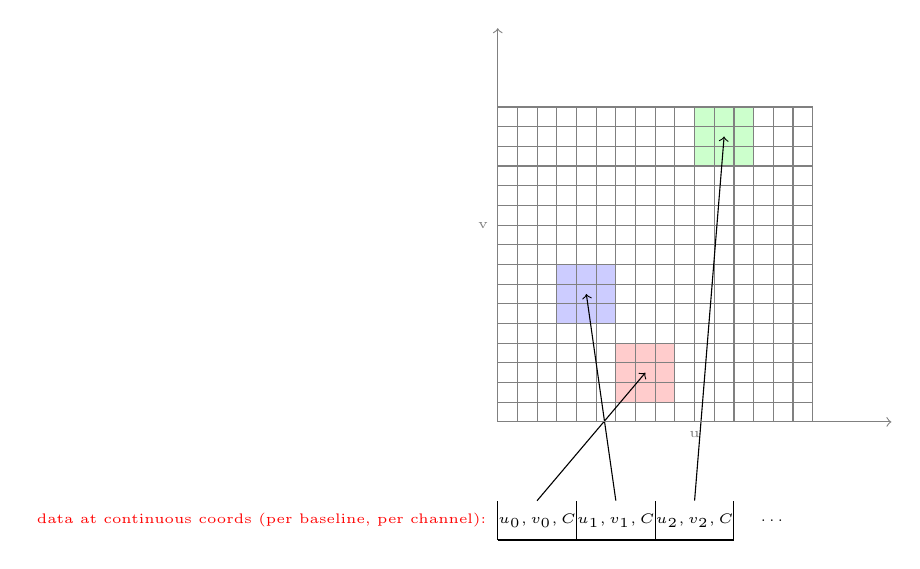
\begin{tikzpicture}[font=\tiny]
    \filldraw[fill=red!20] (4.50,1.75) rectangle (5.25,2.5);
    \filldraw[fill=blue!20] (3.75,2.75) rectangle (4.50,3.50);
    \filldraw[fill=green!20] (5.50,4.75) rectangle (6.25,5.5);
    \draw[step=0.25,gray,thin] (3,1.5) grid (7,5.5);
    \draw[red] node at (0,0.25) {data at continuous coords (per baseline, per channel):};
    \draw node at (6.5,0.25) {\dots};
    \draw[step=1,black] (3,0) grid (6,0.5);
    \draw node at (3.5,0.25) {$u_0,v_0,\mathbb{C}$};
    \draw node at (4.5,0.25) {$u_1,v_1,\mathbb{C}$};
    \draw node at (5.5,0.25) {$u_2,v_2,\mathbb{C}$};
    \draw[->] (3.5,0.5) -- (5-0.125,2.25-0.125);
    \draw[->] (4.5,0.5) -- (4.25-0.125,3.25-0.125);
    \draw[->] (5.5,0.5) -- (6-0.125,5.25-0.125);
    \draw[->,gray] (3,1.5) -- (8,1.5) node[below,pos=0.5]{u};
    \draw[->,gray] (3,1.5) -- (3,6.5) node[left,pos=0.5]{v};
   \end{tikzpicture}
   \caption[Illustration of convolutional gridding]{Each observed visibility (per channel and baseline) is centered at some precomputed coordinate in continuous u,v space and 
    is ``convolved'' with some function $\phi$, which extends only to finite ``full support'' region as illustrated. The result is binned in a regularly spaced grid. 
    This process essentially spreads each visibility out over a larger area in u,v space. It should be clear that this is not the standard convolution 
    operator as defined in Appendix~\ref{chp_DSP}. After all the observed visibilities have been gridded an Inverse Fast Fourier Transform is performed 
    and a correcting function is applied. Each correlation term (or Stokes sum) is typically resampled and transformed to its own image.}
   \label{fig_gridding}
  \end{mdframed}
 \end{figure}
 
 The interpolated measurements taken at the grid points are not known exactly, and normally in interpolation techniques it is 
 hoped that the variance of this error is small as soon as the step size in the resampling process becomes infinitesimally narrow. 
 In the context of radio astronomy the ``significantly oversampled'' criterion is not normally met because of the significant amounts 
 of memory this will require, especially considering the sizes of the arrays currently under construction. Instead, only a 
 \emph{critically sampled} image is usually produced during synthesis. Importantly note that ``critically sampled'' refers to 
 the Shannon-Nyquest sampling criterion:
 \begin{equation}
  \label{eqn_img_sampling}
  \begin{split}
    \text{cell}_l &= \frac{1}{2N_l\Delta{u}}\text{, }\Delta{u}:=\frac{1}{u_{\text{max}}}\\
    \text{cell}_m &= \frac{1}{2N_m\Delta{v}}\text{, }\Delta{v}:=\frac{1}{v_{\text{max}}}\\
  \end{split}
 \end{equation}
 Here $\text{cell}_l$ and $\text{cell}_m$ are the pixel sizes given in degrees (or equivalently arcminutes, arcseconds or radians). $N_l\Delta{u}$ and
 $N_m\Delta{v}$ correspond to the maximum frequencies in the Fourier / measurement space. If the images are 
 sub-sampled (change the equality to $>$) the longest baselines will fall off the uv grid and angular resolution will be lost. 
 
 This sampling criterion alone justifies our statement that the Fourier response of the resampling function should be considered of higher priority
 than the approximation criterion, unlike in other contexts where interpolation quality may be the most important. The energy reduction properties of
 $\phi$ can be stated in terms of maximizing the following integral ratio for all square-integrable $\phi$ functions\footnote{It is possible to
 define another criterion here, for example to promote accurate interpolation over energy concentration. Sze Tan \cite{tan1986aperture} for 
 instance defined this as minimizing the difference between the Direct Transform and the FFT approach}:
 \begin{equation}
  \label{eqn_aliasing_energy}
  \frac{\int_{\text{FOV}}{|[\mathcal{F}\phi](l,m)|^2dS}}{\int_{-\infty}^{\infty}{|[\mathcal{F}\phi](l,m)|^2dS}}
 \end{equation}
 
 To better understand why these repeating or ``aliased sources'' occur in the first place we have to define the gridding operation somewhat more 
 rigorously. Each (discrete) measurement taken by an interferometer in the continuous uv space  is ``convolved'' with a two-dimensional interpolation 
 function in order to create a continuous function. This function is then discretized again onto a set of regular coordinates by a 
 ``bed-of-nails'' function. Mathematically we can say:
 \begin{equation}
  V_{\text{gridded}}[u,v] = [V_{\text{sampled,observed}}(u,v)*\phi(u,v)]\frac{\III(u,v)}{\Delta{u}\Delta{v}}
 \end{equation}
 where $\III$ is the shah function defined as:
 \begin{equation}
  \III(u/\Delta{u},v/\Delta{v})=\Delta{u}\Delta{v}\sum_{j=-\infty,j\in\mathbb{Z}}^{\infty}{\sum_{i=-\infty,i\in\mathbb{Z}}^{\infty}{\delta{(u-j\Delta{u},v-i\Delta{v})}}}
 \end{equation}
 
 Convolution with the Fourier transform of the shah function (composed itself by many band-limited impulses) creates a sum of periodic functions
 in the image domain \footnote{It is useful to note that the Fourier transform of a band-limited (non-zero over a finite range) function, 
 such as a box function, is a function that stretches over an infinite support region}. The result is a periodic field of view that repeats at
 $M\text{cell}_l$ and $N\text{cell}_m$ for an $M\times N$ image (ie. at multiples of the field of view). In practice not all the energy from 
 these replicated fields can be stopped at the edge of the field of view, and this is responsible for the aliasing seen in the images. Further
 truncation of the shah function to represent only a single field of view, as well as the truncation of the convolving function also 
 contribute to the aliasing. It should be understood that the $\psf$ sidelobes from sources outside the field of view that legitimately fall inside
 the field of view are not removed and this will raise the noise levels inside a deconvolved image if the sources responsible for those sidelobes are not
 included in the deconvolved model.
 
 The $\phi$ functions considered here all have the property of \emph{separability}. By this it is implied that $\phi(u,v) = \phi(u)\phi(v)$. We will return
 to a discussion of this later on when discussing w-projection. For now the discussion will focus on functions of one variable.
 
 After aliasing speed becomes a major consideration. Due to the large measurement datasets produced with larger arrays the convolutional resampling process
 has to be fast; the complexity of the resampling step grows as $MC^2$, where C is the support size of the convolution filter. Therefore
 the convolution function $\phi$ is normally pretabulated for a given support size (in grid steps). Additionally it is very important to oversample
 the precomputed $\phi_{\text{filter}}$ to conserve the spatial relation in the measured coherence function and to attain 
 \emph{high dynamic range images}\footnote{Images having a high peak value to noise level}.
 
 To further understand why the filter has to be significantly oversampled (usually dozens of times) consider that interferometers take measurements 
 in the Fourier space, where any rounding operation (or snapping) of the u,v coordinates in either the grid
 or the filter will cause fringe-like decorrelation in the observed sources (think back to the Fourier shift theorem). Th\'evenaz et al. \cite{thevenaz2000image} 
 also points out that $\phi$ must be symmetrical (ie. $\phi{(x)} = \phi{(-x)}$ and $\phi_{\text{filter}}[x] = \phi_{\text{filter}}[-x]$) to preserve 
 the image phase correctly.

 The image phase consideration effectively precludes using nearest-neighbor\footnote{or \textit{cell-summing} techniques as 
 Thompson and Bracewell \cite{thompson1974interpolation} puts it} interpolation. The nearest neighbour technique simply snaps (box function) 
 points close to the grid point into the sum at that point, without any consideration on the visibility's distance from the grid point. Additionally 
 the Fourier transform of the box function is an \emph{infinite} $\sinc$ function.  Due to the fact that the $\sinc$ function slowly ripples out 
 towards infinity it is not a good response when it comes to reducing the unwanted energy from sources that fall outside the field of view.
 
 What makes convolutional gridding a more attractive approach to cell-summing is the fact that the distance between the grid point and the
 measured uv point is taken into consideration when picking a set of convolution weights from the oversampled filter as illustrated in 
 Figure~\ref{fig_filter}. The fractional offset is simply calculated between the nearest regular grid coordinate and measured uv coordinate and is used to pick
 the nearest filter value in the oversampled filter.
 
 \begin{figure}[h]
  \begin{mdframed}
   \centering
   \begin{tikzpicture}[font=\tiny]
    \draw node at ({0*3},0.5) {$\lvert$};
    \draw node at ({0.2*3},0.5) {*};
    \draw node at ({0.4*3},0.5) {*};
    \draw node at ({0.6*3},0.5) {*};
    \draw node at ({0.8*3},0.5) {*};
    \draw node at ({1*3},0.5) {$\lvert$};
    \draw node at ({1.2*3},0.5) {*};
    \draw node at ({1.4*3},0.5) {*};
    \draw node at ({1.6*3},0.5) {*};
    \draw node at ({1.8*3},0.5) {*};
    \draw node at ({2*3},0.5) {$\lvert$};
    \draw node at ({2.2*3},0.5) {*};
    \draw node at ({2.4*3},0.5) {*};
    \draw node at ({2.6*3},0.5) {*};
    \draw node at ({2.8*3},0.5) {*};
    \draw node at ({3*3},0.5) {$\lvert$};
    \draw node at ({3.2*3},0.5) {*};
    \draw node at ({3.4*3},0.5) {*};
    \draw node at ({3.6*3},0.5) {*};
    \draw node at ({3.8*3},0.5) {*};
    \draw node at ({4*3},0.5) {$\lvert$};
    
    \draw node at ({0*3},0) {1};
    \draw node at ({0.2*3},0) {2};
    \draw node at ({0.4*3},0) {3};
    \draw node at ({0.6*3},0) {4};
    \draw node at ({0.8*3},0) {5};
    \draw node at ({1*3},0) {6};
    \draw node at ({1.2*3},0) {7};
    \draw node at ({1.4*3},0) {8};
    \draw node at ({1.6*3},0) {9};
    \draw node at ({1.8*3},0) {10};
    \draw node at ({2*3},0) {11};
    \draw node at ({2.2*3},0) {12};
    \draw node at ({2.4*3},0) {13};
    \draw node at ({2.6*3},0) {14};
    \draw node at ({2.8*3},0) {15};
    \draw node at ({3*3},0) {16};
    \draw node at ({3.2*3},0) {17};
    \draw node at ({3.4*3},0) {18};
    \draw node at ({3.6*3},0) {19};
    \draw node at ({3.8*3},0) {20};
    \draw node at ({4*3},0) {21};
   \end{tikzpicture}
   \caption[Oversampled filter illustration]{Across the literature the definition for ``filter support or window width'' varies considerably. To illustrate the use of the
   terminology in our work a ficticious filter is shown here. Here the padded and oversampled $\phi_{\text{filter}}[x]$ is illustrated for a 3-cell full-support 
   region (half support of 1 to both sides of the centre value), padded with one value on both sides. The filter is 5x oversampled, as indicated by the asterisks
   between the bars, the latter representing the cell-spacing ($\Delta{u}$ for instance) used for the grid. If the measured uv coordinate falls exactly on the nearest grid 
   cell then values 6,11 and 16 are selected as interpolation coefficients. If $\round{(\fracof{(u,v)}m_{\text{oversample factor}})} = 2$ for instance 
   then 8, 13 and 18 are selected for the 3 grid points being ``convolved'' or ``smeared'' onto. In other words: a denser bed of nails is placed over the bed of 
   nails of the grid and the closest set of coefficients for the convolution are selected. Briggs et al. \cite[Lecture 7]{taylor1999synthesis} notes that this discretization
   of $\phi$ will cause a minor replication effect with a very long period of $\frac{m_{\text{oversample factor}}}{\Delta{u}}$ and 
   $\frac{m_{\text{oversample factor}}}{\Delta{v}}$ in the respective u,v directions.}
   \label{fig_filter}
  \end{mdframed}
 \end{figure}
 
 If the last observation about box functions are inverted then we arrive at a partial solution to the problem of selecting a filtering function
 that better limits aliasing energy; convolving with the \emph{infinite} $\sinc$ yields a box response in the image domain. Unfortunately it is 
 impossible to convolve with a infinite function to exactly reconstruct the sought-after box response in the image domain. It is also computationally
 prohibitive to increase the support range of the convolution filter, but without large support sizes the filter's Fourier response does not taper (or 
 ``roll off'') immediately. See Figure~\ref{fig_aliasing_nn_vs_sinc} for a comparative example of the significant difference between nearest neighbor 
 interpolation compared to even just the ordinary $\sinc$ function.
 \begin{figure}[h]
  \begin{mdframed}
    \centering
    \begin{subfigure}[b]{0.35\textwidth}
      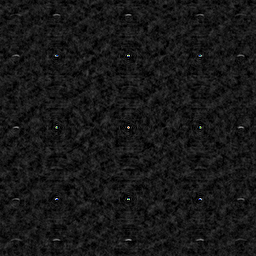
\includegraphics[width=\textwidth]{images/ratt_aa_kernel_demo_nn.png}
      \caption{Nearest neighbor interpolation}
    \end{subfigure}
    \begin{subfigure}[b]{0.35\textwidth}
      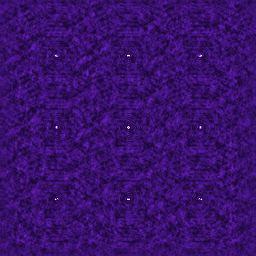
\includegraphics[width=\textwidth]{images/ratt_aa_kernel_demo_larger_support.png}
      \caption{$\sinc$ 8x8 full support}
    \end{subfigure}
    \caption[Alias reduction]{Here a ``grid'' sky model was simulated using MeqTrees\cite{noordam2010meqtrees} and imaged with our imager, first 
    using Nearest Neighbour and then using an ordinary unwindowed $\sinc$ function. Sources that fall slightly outside the field of view are 
    aliased back in when the energy outside the field of view is not limited as expected.}
    \label{fig_aliasing_nn_vs_sinc}
  \end{mdframed}
 \end{figure}
 
 To address this problem the literature is filled with alternative windowing functions to the truncation window, of which 
 the Kaiser-Bessel window proposed by Jackson et al. \cite{jackson1991selection} yields very good results. 
 Offringa et al. \cite{offringa2014wsclean}\footnote{Special thanks goes to Andr\'e Offringa for sending me a snipped of code
 where he implemented this filtering and useful discussions around this topic} used this filter in their implementation of a 
 w-stacking (explained later) imager to great success. The Keiser-Bessel window is defined as:
 \begin{equation}
  \frac{1}{W}I_0(\beta\sqrt{1-(2x/W)^2})
 \end{equation}
 Where W is the full support of the convolution filter. See Jackson et al.\cite{jackson1991selection} for the tabulated constants used 
 for $\beta$.

 An alternative to using a windowed $\sinc$ function is to use a prolate spheriodal function. It is also widely employed in 
 astronomical imagers. The Spheriodal functions have the property we're looking for, in that most of their energy is concentrated 
 over the central part of the function, as measured by a weighted variant of Equation~\ref{eqn_aliasing_energy}. This is proven generally by 
 Donald Rhodes \cite{rhodes1970spheroidal}. A later analysis by Frederic Schwab \cite{schwab1984optimal} confirms the relatively good 
 performance of the spheriodal functions compared with many others as an anti-aliasing filter. The prolate spheriodal is defined as 
 for the special case that $\alpha=0$:
 \begin{equation}
  |1-(2x/W)^2|^\alpha\psi_{\alpha0}(0.5\pi W,2x/W)
 \end{equation}
 
 Here $W$ is again the full support of the the convolution filter and $x$ increases in steps of $\Delta{u}$. When $\alpha>0$ a 
 weighted energy concentration ratio is maximized instead. The $\psi_{xy}$ function is the one defined by Donald Rhodes \cite{rhodes1970spheroidal}.
 Its definition alone is well beyond the scope of this discussion, and in fact it is quite difficult to compute for arbitrary support and
 oversampling parameters.
 
 After taking the Fourier transform the tapering effects of $\phi$ may optionally be corrected for by point-wise division with the Fourier transform of
 $\phi$. This does not completely eliminate $\phi$ from the resulting expression, but has the effect of flattening the response of the pass band (removes the
 tapering towards the edges of the image), but at the same time increasing the amplitudes of the aliasing-sidelobe responses.
 
 Measuring the remaining energy outside the grid-corrected image, Jackson et al.\cite{jackson1991selection} shows that the Keiser-Bessel-windowed $\sinc$ achieves 
 very similar performance to the Gaussian and Prolate Spheriodal Function for small (preferable) support regions and similar performance to the 
 prolate spheriodal for larger windows, whilst being considerably easier to compute than the latter. One possible downside to windowed sinc functions
 are their inability to reproduce a constant function as Th\'evenaz et al. \cite{thevenaz2000image} points out. A synthesized image with a non-zero 
 mean will appear either too light or too dark when compared to a model image. It is unclear if the prolate spheriodal function suffers from the same
 problem. Th\'evenaz et al. also points out that the sinc introduces blockiness in the image.
 
 Lastly it is necessary add (though this is unrelated to the discussions above) that both the Direct Fourier Transform and Fast Fourier Transform approaches
 have to scale the field of view of the image according to the cell size and number of pixels in the image. In the Fast Fourier Transform approach this is 
 achieved by scaling the measurement domain's u,v coordinates (measured in $\text{cycles}.\text{m}^{-1}.\text{rad}^{-1}$) such that, when inverted, the image
 has the desired field of view. To achieve this we use the \emph{similarity} property of the FFT:
 \begin{equation}
  \alpha^{-n}F(x/\alpha) \rightleftharpoons f(\alpha x)
 \end{equation}
 Here $n$ depends on the dimensionality of the Fourier transform. If the desired field of view (measured in radians, centred at the field centre) is multiplied to 
 each sampled u,v coordinate then the synthesized image will have a field of view ranging between $-0.5\text{cell}_{l}N_l\leq l_{\text{deg}}\leq0.5\text{cell}_{l}N_l$ and 
 $-0.5\text{cell}_{m}N_m\leq m_{\text{deg}}\leq0.5\text{cell}_{m}N_m$. It is further important to note that, by convention, the gridded visibilities are shifted before Fourier 
 transform such that the 0 frequency component (``DC'' component) is at the centre of the grid and the corresponding centre of the 
 observed field on the image is at the centre pixel of the image.
 
 To summarize the convolutional gridding process is shown in Figure~\ref{fig_synth_pipeline}.
 \begin{figure}[h]
  \begin{mdframed}
    \centering
    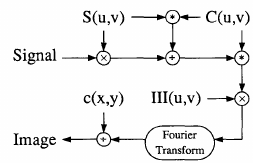
\includegraphics[width=0.4\textwidth]{images/convolutional_gridding_flow.png}
    \caption[Synthesis using convolutional gridding]{Here the classic synthesis by convolutional gridding and Inverse Fast Fourier transform is shown.
    The signal (u,v domain) is multiplied by a sampling function (and optionally weighted by the computed and tapered density function). Then it is convolved
    and resampled onto the regular grid, Fourier transformed and optionally grid-corrected by point wise division. Courtesy of Jackson et al.\cite{jackson1991selection}}
    \label{fig_synth_pipeline}
  \end{mdframed}
 \end{figure}
 
\section{Wide field distortions and the problem of non-coplanar baselines}
Up to this point the discussion on employing the Fast Fourier Transform to invert interferometer measurements and discretize the sky has relied on the assumption
that the the field of view under consideration can be well-approximated by a tangent projection plane. When synthesizing an image over a larger field of view
this assumption is broken. This is especially true for lower-frequency instruments such as LOFAR. Much of the remainder of this 
chapter will focus on the effects the additional phase delay term $w(n-1)$ in the RIME has on the synthesized image. The effect has been extensively studied over 
the past two decades and is quite well understood. Our discussion will include the proposed solutions in the literature and will draw extensively on the works of 
Rick Perley \cite[Lecture 19]{taylor1999synthesis}\footnote{A word of thanks to Rick for his insightful discussions on the problem and clarification on his 
tangent facet imaging approach in late 2014}, Tim Cornwell and 
Rick Perley \cite{cornwell1992radio}, Cornwell, Golap and Bhatnagar \cite{cornwell2008noncoplanar}, Kogan and Greisen \cite{aipsfaceting}, and 
Cyril Tasse \cite{tassefaceting}\footnote{This document is an internal memorandum explaining some of the ideas exploited in this work. A great debt of gratitude 
is owed to Cyril for compiling this discussion on facet and hybrid facet imaging.}.

The widefield effect arise due to the combination of two errors:
\begin{enumerate}
 \item Firstly the array geometry in significantly non-coplanar arrays will lead to w-values that cannot be ignored. Similarly the non-East-West baselines
 in arrays will not remain coplanar over the duration of an observation. These will be rotated up into the w direction as the Earth rotates, even if the physical 
 array layout is on a very flat plane (as is true for the EVLA for example).
 \item Secondly the image projection geometry worsens the signal phase difference between antennae. The distance between the planar projection of the sky and the 
 celestial sphere (or unit radius ``sky dome'') cannot be ignored far away from the tangent point of the image. This error in distance is expressed 
 as $n-n_0$ where $n = \sqrt{1-l^2-m^2}$ at the correct position of the source on the celestial sphere, and $n_0=\sqrt{1-l_0^2-m_0^2}$ is the 
 tangent point / projection pole of the image produced using the Fast Fourier Transform, assuming this projection is the ordinary orthogonal 
 projection of the sphere onto to the image.
\end{enumerate}
As Rick points out this phase difference is not a physical delay in the strictest sense of the word, but arise merely because of the geometry of the array and coordinate
systems. In essence it arises because the field of view is too wide, or it is sampled with a tilted interferometer or both problems arise simultaneously. The effects 
are combined as $w(\sqrt{1-l^2-m^2} - \sqrt{1-l_0^2-m_0^2})$ where $\sqrt{1-l_0^2-m_0^2} = 1$ if the projection pole is at the same coordinate as the centre
of the field being observed (which we take to be true for the remainder of the discussion). Because the phase propagation term $\tau = \frac{\vec{b}\cdot\vec{s}}{c}$ as 
shown in Figure~\ref{fig_interferometer} depends on the distance a source is away from the delay tracking centre at $\vec{s}_0$ it will continuously change during the course 
of an observation. As the baselines are rotated with respect to a fixed position in the sky, the apparent position of sources in the image will move as the earth rotates. To see why 
the latter statement is true from a pure mathematical standpoint consider again the Fourier Shift Theorem:
\begin{equation}
 g(x-\Delta) \rightleftharpoons G(f)e^{-2\pi if\Delta}
\end{equation}
This theorem says that adding a delay term through multiplication by a complex exponential in the Fourier (measurement) domain will serve to shift values in the 
signal (sky/image) domain. In this context the effect is somewhat more complicated because sources closer to the tracking centre of the field are not as affected 
by this shift as those further away from the field centre. Refer to Figure~\ref{fig_wide_field_error} for an illustration of the two terms: $w$ and $(n-1)$.

\begin{figure}[h]
  \begin{mdframed}
    \centering
    \begin{subfigure}[b]{0.70\textwidth}
     \centering
     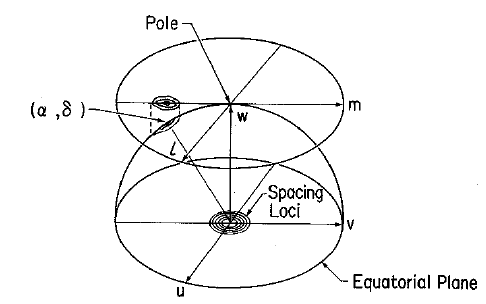
\includegraphics[width=\textwidth]{images/source_projection_onto_image_plane.png}
     \caption{}
    \end{subfigure}
    \begin{subfigure}[b]{0.45\textwidth}
      \centering
      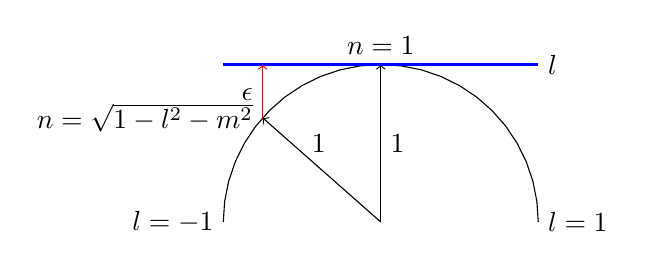
\begin{tikzpicture}
	\draw [black, domain=0:180] plot ({2*cos(\x)}, {2*sin(\x)});
	\draw [black, ->] (0,0) -- (0,2);
	\draw [black, ->] (0,0) -- ({-0.75*2},{sqrt(4-(-0.75*2)*(-0.75*2))});
	\node [above] at (0,1*2) {$n=1$};
	\node [right] at (0,0.5*2) {$1$};
	\node [right] at (-0.5*2,0.5*2) {$1$};
	\node [left] at ({-0.75*2},{sqrt(4-(-0.75*2)*(-0.75*2))}) {$n=\sqrt{1-l^2-m^2}$};
	\draw [blue,thick] (-2,2) -- (2,2);
	\draw [red, ->] ({-0.75*2},{sqrt(4-(-0.75*2)*(-0.75*2))}) -- ({-0.75*2},2);
	\node [left] at ({-0.75*2},{sqrt(4-(-0.75*2)*(-0.75*2))+0.15*2}) {$\epsilon$};
	\node [right] at ({1*2},{1*2}) {$l$};
	\node [right] at ({1*2},{0*2}) {$l=1$};
	\node [left] at ({-1*2},{0*2}) {$l=-1$};
      \end{tikzpicture}
      \caption{Error between the orthogonal planar FFT approximation to the sky and the correct position on the celestial sphere}
    \end{subfigure}
    \begin{subfigure}[b]{0.45\textwidth}
      \centering
      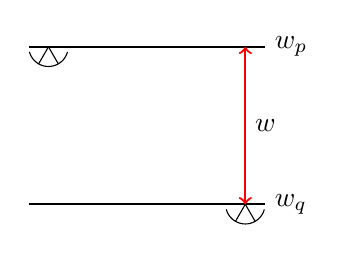
\begin{tikzpicture}
	\draw [black,thick] (0,2) -- (3,2);
	\draw [black,thick] (0,0) -- (3,0);
	\draw [black, domain={180+15}:{360-15}] plot ({(cos(\x)+1)*0.25}, {(sin(\x))*0.25+2});
	\draw [black] ({0.25*0.5},{2 - sqrt(0.25*0.25*(1-0.5*0.5))}) -- ({0.25},{2});
	\draw [black] ({0.25*1.5},{2 - sqrt(0.25*0.25*(1-0.5*0.5))}) -- ({0.25},{2});
	\draw [black, domain={180+15}:{360-15}] plot ({(cos(\x)-1)*0.25+3}, {(sin(\x))*0.25});
	\draw [black] ({3-0.25*0.5},{0 - sqrt(0.25*0.25*(1-0.5*0.5))}) -- ({3-0.25},{0});
	\draw [black] ({3-0.25*1.5},{0 - sqrt(0.25*0.25*(1-0.5*0.5))}) -- ({3-0.25},{0});
	\draw [red,thick,<->] ({3-0.25},{0}) -- ({3-0.25},{2});
	\node [right] at ({3-0.25},{1}) {$w$};
	\node [right] at ({3},{2}) {$w_{p}$};
	\node [right] at ({3},{0}) {$w_{q}$};
      \end{tikzpicture}
      \caption{Delay in signal propagation between antennas in an array-based telescope at some instant in time}
    \end{subfigure}
    \caption[Widefield phase delay]{In (a) the projected position of a source on the sky dome onto the plane tangent to the projection pole is shown. The baseline tracks
    are concentric circles exactly parallel to the Earth's equator in the case of East-West arrays. Image adapted from A. Richard Thompson \cite[Lecture 2]{taylor1999synthesis}. 
    The combined propagation delay of emission from sources far away from the telescope pointing centre is a combination
    of the error between the planar approximation and the celestial sphere (b) and the phase difference between pairs of antennae in the telescope
    pointing direction as illustrated as shown in (c). The total phase error is expressed as $w(n-1)$. The multiplicative effect of this w-term becomes a
    significant problem in large non-East-West antenna arrays, where the baselines between the furthest-separated antenna pairs become significantly non-coplanar 
    as the Earth rotates.}
    \label{fig_wide_field_error}
  \end{mdframed}
\end{figure}

To add to this problem the difference in the w-term between the antennae increases for observations at lower elevation angles (ie. those observations near the horizon). To see why that
is true consider that the baseline tracks of observations near NCP consists almost entirely of level concentric circles. As the declination (and elevation) angle is decreased 
more and more of the circles have non-zero w-components, to the point that their projection onto the uv plane becomes a straight line at $\delta=0$. This last observation
gives us an estimation for the absolute of the maximum w-value the observation may contain\footnote{This is a conservative estimate for imaging at lower elevation angles (near the horizon),
the maximum w-value will be significantly less near Zenith}, as well as the sample spacing needed to satisfy the Shannon-Nyquest sampling constraint, 
as A. Richard Thompson \cite[Lecture 2]{taylor1999synthesis} notes (refer to Figure~\ref{fig_max_baseline} for an illustration of the argument):
\begin{equation}
 \label{eqn_wmax}
 \begin{split}
  w_{\text{max}} &\approx |\frac{\vec{b}_{\text{max}}}{\lambda}|\\
  \text{cell}_l &= \text{cell}_m = \text{cell}_n \approx 0.5\frac{\lambda}{|\vec{b}_{\text{max}}|}\\
 \end{split}
\end{equation}

\begin{figure}[h!]
  \begin{mdframed}
    \centering
    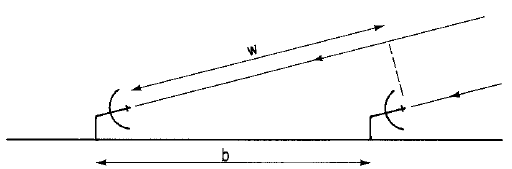
\includegraphics[width=0.8\textwidth]{images/max_w.png}
    \caption[Maximum w-estimation at low azimuth angle observation]{When sources are observed at low elevation (or similarly at low declinations) angles,
    for instance those sources rising or setting at the horizon, the delay between the two observing antennae are maximized and by implication w since w is usually
    defined to point towards the tracking centre of the field. Image courtesy of A. Richard Thompson \cite[Lecture 2]{taylor1999synthesis}}
    \label{fig_max_baseline}
  \end{mdframed}
\end{figure}

The resulting effect on the apparent position of a source over time from this declination-dependent increase in w is plotted in Figure~\ref{fig_position_shifts_and_decorrelation}. We have 
additionally imaged a simulated sky model consisting of point sources in a grid pattern to show the resulting decorrelation in the resolution of sources far from the delay tracking centre 
and their corrected version in the same figure.

\begin{figure}[ht!]
  \begin{mdframed}
    \centering
    \begin{subfigure}[b]{0.62\textwidth}
      \centering
      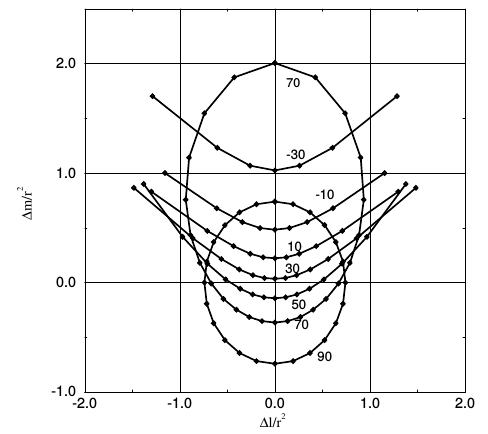
\includegraphics[width=\textwidth]{images/apparent_position_shifts.png}
      \caption{}
    \end{subfigure}
    \begin{subfigure}[b]{0.49\textwidth}
      \centering
      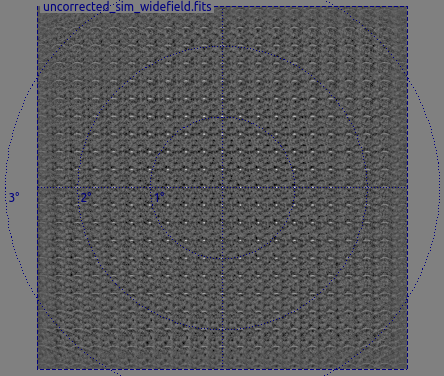
\includegraphics[width=\textwidth]{images/widefield_meerkat.png}
      \caption{}
    \end{subfigure}
    \begin{subfigure}[b]{0.49\textwidth}
      \centering
      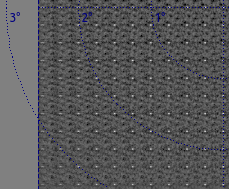
\includegraphics[width=\textwidth]{images/widefield_corrected_meerkat.png}
      \caption{}
    \end{subfigure}
    \caption[Apparent shift in source position and resulting decorrelation]{In (a) the apparent source positions for sources less than one radian from field centre in 
    several hourly-interval snapshots on the VLA at 7 declinations are plotted by Rick Perley \cite[Lecture 19]{taylor1999synthesis}. The dots of the zero hour angle is indicated on the vertical 
    axis. The angular position errors here are measured, where $r^2=l^2+m^2$. In (b) a simulated gridded sky (without effects of the antenna beam or noise included) is 
    synthesized as a dirty image using the regular planar transform as described in the previous section. In (c) the dirty map is synthesized again, here it is 
    corrected using the w-projection technique explained later on. The point sources near the edge of the field are no longer smeared.}
    \label{fig_position_shifts_and_decorrelation}
  \end{mdframed}
\end{figure}

To correct this effect one may consider employing a three dimensional Fourier transform. Rick \cite[Lecture 19]{taylor1999synthesis} shows that the 
image along the sky plane can be related to the intensity cube derived by a three-dimensional Fourier transform, assuming n as an independent variable. 
The sky then is defined by all the points in the transformed cube that lie on a shifted unit sphere. This relation is also informative about the possible 
effects of the sampling function; the $\psf$ is not only convolved with the points on the sky sphere, but the surrounding areas in the cube.

Such a full three dimensional transform is not a practical solution considering the sheer amount of memory that would be required to form several layers,
each the size of the image and considering the computational costs because the cube layers in the $n$ dimension must be computed using a direct Fourier 
transform to overcome the aliasing effects introduced by the longest baseline. Instead Rick \cite[Lecture 19]{taylor1999synthesis} mentions 2 more 
solutions to the problem and Cornwell et al. \cite{cornwell2008noncoplanar} later come to a third solution:
\begin{enumerate}
 \item Warped snapshot imaging. If the observation time is sufficiently short, all the baselines of the array remain relatively coplanar\footnote{within a 
 fraction of the cell size in n}. By neglecting the w-term a small distortion is introduced in the apparent position of sources This becomes the determinant
 factor in deciding the maximum observation time for each snapshot image. Due to the continuous rotation of the tangent image plane in this solution it is necessary
 to accurately interpolate the cell coordinates between snapshots. This latter operation becomes the dominant factor in snapshot imaging (see Rick Perley \cite[Lecture 19]{taylor1999synthesis}
 and Cornwell, Voronkov and Humphreys \cite{cornwell2012wide} for details).
 \item Facet imaging \footnote{Or a ``fly's eye'' imaging approach as Bill Cotton labels it.}. The varying w term can be assumed to be near-constant across a narrow field of view, therefore a 
 wide field of view can be broken up into several narrow field images, each limiting the distance between the approximating plane and the celestial sphere. There are both \emph{non-coplanar} and \emph{coplanar}
 faceting approaches, as well as the appropriate transforms and coordinate reprojections in the measurement and image spaces to accompany these two variants. The details will be 
 outlined in the next few sections.
 \item W-projection \cite{cornwell2008noncoplanar} and W-stacking \cite{offringa2014wsclean}. The w-term can be thought of as a w-dependent convolution
 in the Fourier domain. By convolving each visibility with the Fourier transform of $w(n-1)$ during the gridding process it is possible to re-introduce 
 this multiplicative phase term in the image domain. Similarly it is also possible to divide the sky image up into several w-dependent layers and point-wise
 multiply the w phase screen into each layer in image space, reducing the planes into a single image afterwards (w-stacking).
\end{enumerate}

The approaches above attempt to either drive $w$ down to zero (snapshots or w-projection) or drive $(n-1)$ down to zero (facet imaging). There is no reason why
the approaches cannot be combined, for instance Cornwell, Voronkov and Humphreys \cite{cornwell2012wide} combine w-projection and traditional snapshot imaging, while
Offringa et al. includes a Zenithal w-snapshot synthesis mode in their work. Our work on the other hand focus on combining traditional facet imaging and w-projection, 
in order to harness some of the positive aspects of both approaches.

\section{Non-coplanar facet imaging}
The goal in faceting is to approximate a wider field of view by many small narrow field images. Rick Perley and Tim Cornwell \cite{cornwell1992radio} proposes a 
polyhedron-like faceting approach, where each narrow-field facet is tangent to the celestial sphere at its own phase tracking centre $(l_i,m_i)$. We will classify
this basic faceting approach to be non-coplanar uvw-space faceting, because each facet lies on its own tangent plane and the coordinate transformations
necessary for this tilted polyhedron approach are done on the uvw-coordinates (measurement coordinates) and not in the image space.

Just as with regular narrow field imaging the phase term $e^{-2\pi i \vec{b}\cdot(\vec{s}-\vec{s}_0)}$ are taken relative to a delay tracking centre in the direction
$\vec{s}_0$. Synthesizing an image with a new phase tracking centre, $\vec{s}_i$, it is only necessary to employ the shift theorem. This follows naturally from the
RIME (simplified here). Let $(l_\Delta,m_\Delta,n_\Delta) = (l_i-l_0,m_i-m_0,n_i-n_0)$, then:
\begin{equation}
  \label{eqn_faceting}
  \begin{split}
    V(u,v,w)&\approx\int{\int{B(l-l_i,m-m_i,n-n_i)e^{-2{\pi}i[u(l-l_i)+v(m-m_i)+w(n-n_i)]}\frac{dldm}{n}}}\\
    &\approx\int{\int{B(l-l_i,m-m_i,n-n_i)e^{-2{\pi}i[u(l-l_0-l_\Delta)+v(m-m_0-m_\Delta)+w(n-n_0-n_\Delta)]}\frac{dldm}{n}}}\\
    &\approx\left[\int{\int{B(l-l_0,m-m_0,n-n_0)e^{-2{\pi}i[u(l-l_0)+v(m-m_0)+w(n-n_0)]}\frac{dldm}{n}}}\right]e^{2{\pi}i[ul_\Delta,vm_\Delta,wn_\Delta]}\\
  \end{split}
\end{equation}

In words this says that the telescope can be electrically steered to take measurements with respect to a new phase centre by multiplying each known measurment in
the database by a complex exponential. However, the intensity measurements are still the ones measured with respect to the original u,v,w coordinates. The result of
the latter observation is that the sky is projected onto facet planes that are tangent to the original phase tracking centre, $(l_0,m_0)$ and not the new phase 
tracking centres, $(l_i,m_i)$.

Rick shows that only employing a phase shift per visibility without regard of the tangency of the resulting facets will require the creation of many more facets 
further from the original field centre. This is illustrated in Figure~\ref{fig_non_rotated_facets} Employing a small angle approximation to estimate $(n-1)$ and applying the critical sampling criteria estimated in 
Equation~\ref{eqn_wmax}, Rick estimates the maximum undistorted field of view to be:
\begin{equation}
 \theta_{\text{max}} \approx \frac{\lambda}{2|\vec{b}_{\text{max}}|\theta_i}
\end{equation}
where $\theta_i$ is the angle to the new phase centre.

\begin{figure}[h]
  \begin{mdframed}
    \centering
    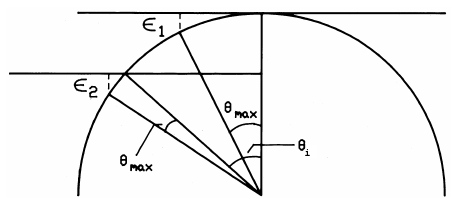
\includegraphics[width=0.7\textwidth]{images/non_rotated_faceting.png}
    \caption[Faceting without regard of tangency]{By only phase steering the visibilities to new phase centres without tilting the u,v,w coordinates
    to correspond to the new phase tracking centre significantly reduces the achievable field of view. Here instead each facet is parallel to the 
    original tangent plane. As the new phase tracking centre is taken further away from the original phase tracking centre the effective facet size must be
    shrunk down to achieve a comparable projection error at the edge of the synthesized facets. Image adapted from Rick Perley \cite[Lecture 19]{taylor1999synthesis}}
    \label{fig_non_rotated_facets}
  \end{mdframed}
\end{figure}

In order to make each facet tangent to the celestial sphere at $(l_i,m_i)$ it is necessary to employ the rotation matrices from Equation~\ref{EQN_LEFTHANDED_SYSTEM}
to compute new u',v',w' coordinates \emph{after} the visibilities have been phase shifted using the old u,v,w coordinates.
\begin{equation}
 \left[\begin{array}{c}
	u'\\
	v'\\
	w'\\
       \end{array} \right] = R(\alpha_i,\delta_i)R^{T}(\alpha_0,\delta_0)\left[\begin{array}{c}
										u\\
										v \\
										w \\
									      \end{array}
									\right]
\end{equation}

By ensuring the facets are tangent to the new phase centres one in effect ensures that the height difference between the sky and the projected facet remains
comparable between corresponding pixels. Rick estimates that such a polyhedron approach achieves a field of view estimated by:
\begin{equation}
 \theta_{\text{max}} \approx \frac{\sqrt{\lambda}}{\sqrt{|\vec{b}_{\text{max}}|}}
\end{equation}

Using a polyhedron faceting approach is clearly an improvement over the naive phase steering approach if enough facets are created to satisfy the sampling 
criterion. To determine how many facets are required we first have to define the phase error as (refer back to Figure~\ref{fig_wide_field_error}):
\begin{equation}
\label{eqn_phase_error}
\xi_{\text{max}}:=\frac{2{\pi}w_{\text{max}}\epsilon}{{\lambda_{\text{min}}}} \text{, }\epsilon:=\sqrt{1-l^2-m^2} - \sqrt{1-l_0^2-m_0^2} \text{ and ideally } 0{\leq\xi\ll}1
\end{equation}

Then we derive an indication of the number of facets needed to limit this w-dependent phase error between the celestial sphere and orthogonally projected 
facets (linearly spaced) at the corner of each facet:
\begin{equation}
N_{\text{facets}} = \frac{\max{(\theta_l,\theta_m)}}{2\cos^{-1}{\left[\sin{(\delta_0 + \theta_l/2)}\sin{\delta_0} + \cos{(\delta_0 + \theta_l/2)}\cos{\delta_0}\cos{(\theta_m/2)}-\frac{\lambda_{\text{min}}\xi}{2{\pi}w_{\text{max}}}\right]}}
\end{equation}

Here the half facet size (in l and m) is given as $\theta_{l_f}/2 = \theta_l/(2N_{\text{facets}})$ and $\theta_{m_f}/2 = \theta_m/(2N_{\text{facets}})$ respectively. The arc subtended by the angle to the corner of the facet has 
length $\cos{(\theta_{l_f}/2)}\cos{(\theta_{m_f}/2)}$ using the spherical rule of cosines and assuming a unit celestial sphere and orthogonal u and v bases. The angle to the corner of the image is a small number, so 
we might as well just use the small angle approximation.

For reference a sketch algorithm for facet synthesis (backwards step) is given in Algorithm~\ref{alg_polyhedron_faceting_sketch}. The forward
step will work roughly in reverse. The faceting transformations in practice are combined with the gridding algorithm.
\begin{algorithm}
  \begin{algorithmic}
  \STATE {Let $g_f^b$ be all-zero complex $n \times m$ pixel grids, one per continuum band (spectral window), $b$, of facet $f$}
  \STATE {Given $(\alpha_0,\delta_0)$, the original field centre of the telescope (assuming field centre and phase tracking centre are the same)}
  \FORALL {facet centres $(\alpha_i,\delta_i)$}
    \FORALL {channels $c$ in the continuum image band}
      \STATE {Let uvw be a set of $M$ measurement coordinate triples}
      \STATE {Let uvw' be a set of rotated uvw coordinates, applying $R(\alpha_i,\delta_i)R^{T}(\alpha_0,\delta_0)$}
      \STATE {Let vis be a set of $M$ measurements, each corresponding to a uvw triple}
      \STATE {Obtain projected (assumed orthogonal/``SIN'') $(l_i,m_i,n_i)$ and $(l_0,m_0,n_0)$ coordinates}
      \STATE {Let $\lambda$ be the channel wavelength}
      \STATE {Let $p_f=\exp{(2\pi i/\lambda[u(l_i-l_0)+v(m_i-m_0)+w(n_i-n_0)])}$} 
      \STATE {Let vis' = vis * $p_f$, by element-wise multiplication}
      \STATE {Call convolve\_grid($g_f^b$,vis',uvw')}
    \ENDFOR
  \ENDFOR
  \STATE{Invert $g_f^b$ using shifted Inverse FFT}
  \end{algorithmic}
  \caption{The Perley polyhedron faceting algorithm (sketch)}
  \label{alg_polyhedron_faceting_sketch}
\end{algorithm}

For reference the relationship between the celestial and projected image plane coordinates are given here, where
$\alpha_p,\delta_p$ is the tangent point\footnote{The tangent point is assumed to be the same as the phase reference 
centre for the orthogonal projection, which is a special case of an Azimuthal projection. For more details see the 
AIPS convention \cite{aipsnonlinearcoords} and Calabretta and Greisen \cite{calabretta2002representations}}:
\begin{equation}
 \begin{split}
  l &= \cos{\delta}\sin{(\alpha-\alpha_p)}\\
  m &= \sin{\delta}\cos{\delta_p}-\cos{\delta}\sin{\delta_p}\cos{(\alpha-\alpha_p)}\\
  n &= \sqrt{1-l^2-m^2}\\
 \end{split}
\end{equation}

For our work we assume the projection is the orthogonal coordinate system specified here. It is well worth noting 
that the orthogonal projection of sources is not accurate for large fields of view, as noted by Calabretta and Greisen 
\cite{calabretta2002representations}.

Another important remark is that the resolution of each facet image is not arbitrary, but is subject to the same Nyquest sampling 
criteria outlined for regular images in Equation~\ref{eqn_img_sampling}.
\section{Coplanar facet imaging}
One of the biggest downfalls to Rick's non-coplanar faceting approach is that the minor cycle deconvolution becomes very complicated; the measurement
coordinates are rotated and because rotations are preserved by the Fourier transform, the $\psf$ is also rotated. Since the $\psf$ is not necessarily 
symmetric each facet has its own $\psf$. Combining the CLEAN components in the subtraction phase will also require careful consideration during the minor cycle.

One way around this problem would be to re-project each non-coplanar facet into a single plane after synthesis (ie. in the image-space). Doing the necessary
re-projections and inevitable (and expensive) corrections for the areas where the facets overlap can be done through astronomical mosaicking software packages such as the
Montage \cite{jacob2004montage} suite of tasks. It is also possible to do the necessary rotation and sheering operations in the u,v space through 
linear\footnote{A linear operation is required to conserve the Fourier relation between the sky and visibilities} operations given by 
Sault et al. \cite[Appendix A]{sault1996approach}. Although the major cycle, would, in turn require that the regular visibilities be read off all
the constituent facets' Fourier transforms the latter approach of re-projecting the u,v coordinates and phase steering is no more expensive than the backward 
step.

Another way to do (approximate) coplanar faceting is to consider taking the phase error in Equation~\ref{eqn_phase_error} into account while gridding the facets.
One such strategy to include $w\epsilon$ per gridded visibility is to Taylor expand the term to a first order approximation around the original phase centre. The 
first order approximation leads to a remarkable transformation for u and v as pointed out by Leonid Kogan and Eric Greisen \cite{aipsfaceting}:
\begin{equation}
 \begin{split}
  \epsilon&\approx \left[\frac{\partial \epsilon}{\partial l}\right]_{l_i}(l - l_i) + \left[\frac{\partial \epsilon}{\partial m}\right]_{m_i}(m - m_i) + \dots\\
  &\approx \frac{1}{\sqrt{1-l_i^2-m_i^2}}(l_i(l - l_i) + m_i(l - l_i)) + \dots\\
 \end{split}
\end{equation}
Substituting into Equation~\ref{eqn_faceting} they obtain:
\begin{equation}
 \begin{split}
  V(u,v,w)&\approx\int{\int{B(l-l_i,m-m_i,n-n_i)e^{-2{\pi}i[u'(l-l_i)+v'(m-m_i)]}\frac{dldm}{n}}}\\
  u'&=u - w\frac{l_i}{\sqrt{1-l_i^2-m_i^2}}\\
  v'&=v - w\frac{m_i}{\sqrt{1-l_i^2-m_i^2}}\\
 \end{split}
\end{equation}
The first order approximation approach may also be thought of as reducing the projection error, $\epsilon$, to near zero, provided the new facet is small enough. 
The resulting facets are thus all (nearly) parallel. Since the w-term is merely an approximation we assumed the phase steering term is the same as in the original
polyhedron-faceting algorithm. Bill Cotton\cite{obitfacetclean}\footnote{A word of thanks goes to Bill Cotton for useful discussions on facet imaging in late 2014} 
uses this coplanar facet synthesis method in a joint major-minor cycle deconvolution approach in Obit.

As one would expect the first order approximation still breaks down if the facet edges are several degrees away from the facet phase centre.
Unfortunately the second degree terms cannot easily be separated as was done for $u'$ and $v'$ and would require using a convolution in the Fourier domain
in order to multiply the approximate $w(n-n_i)$ phase screen into the image domain. As Cyril \cite{tassefaceting} points out one can additionally improve the approximation
by fitting a smooth polynomial through w. Unfortunately, it should be noted that this implies that a set of w-planes have to be stored per facet, so one might
as well do a hybrid approach between faceting and traditional w-projection, although the W-kernels themselves arguably is smoother for the first approach. The last
statement will become clearer once the original w-projection algorithm is discussed. After discussing w-projection we compare the error in doing a first 
order expansion compared to a full w-projection approach. 
\section{The W-projection algorithm}
As already mentioned the core idea in w-projection is to multiply the intensity distribution by a w-dependent phase screen. Cornwell, Golap and Bhatnagar \cite{cornwell2008noncoplanar}
notes that observations with non-zero $w$ coordinate can be related to a single observation plane (with $w=0$) through convolution in the measurement domain. To make this
more concrete consider that a measurement of the sky brightness distribution, $B(l,m)$, is modulated by fringes defined by $\mathfrak{w}_w := e^{-2\pi i w(\sqrt{1-l^2-m^2}-\sqrt{1-l_0^2-m_0^2})}$ if the 
w-dependent $\mathfrak{w}$ term is separated from the usual phase term. Unlike in faceting this additional phase term cannot be taken out of the integral due to the dependence on $l$ and $m$. Instead
we consider employing the convolution theorem to multiply the phase term into the measurement integral:
\begin{equation}
 \begin{split}
        V(u,v,w)&\approx\int{\int{B(l,m)e^{-2{\pi}i[u(l-l_i)+v(m-m_i)]}e^{-2{\pi}i[w(n-n_i)]}\frac{dldm}{n}}}\\
		&\approx\int{\int{B(l,m)e^{-2{\pi}i[u(l-l_i)+v(m-m_i)]}\mathfrak{w}_w(l,m)\frac{dldm}{n}}}\\
		&\approx V(u,v,w=0)*\mathfrak{W}_w(u,v)\\
	V(u,v) * \mathfrak{W}_w(u,v) &\rightleftharpoons B(l,m)\mathfrak{w}_w(l,m)\\
 \end{split}
\end{equation}

Because of the w dependence of $\mathfrak{w}$ this convolution is done while gridding (and degridding) the visibilities, just as is done with the regular 
anti-aliasing filter, only now the filter must have complex values (as provisioned for in Equation~\ref{eqn_interp_op}). Just as with FFT-based narrow 
field imaging, it is still important to include the response of the anti-aliasing function. There is no obvious closed-form expression for the 
Fourier transform of $\mathfrak{w}_w\mathcal{F}[\phi]$ for arbitrary $\phi$ functions, so the Fourier transform of the combined function must be precomputed 
for several values of $w$. During convolution the nearest $w$-layer is picked depending on the value of the $w$ coordinate. Aside from this minor modification 
of the interpolation step, the rest of the previous discussion remains valid.

The immediate concern is determining how many $w$-planes must be precomputed. Here it is useful to note that the difference in the $w(n-1)$ during the
observation is responsible for the decorrelation in source brightness as explained earlier, one would therefore hope to minimize $\xi_{\text{max}}$ by introducing
$N_{\text{planes}}$ different $w$-planes (here assumed to be linearly separated\footnote{For arrays that are dense in the core region it may be better to consider
a denser distribution of planes for lower w}) between the $w_{\text{max}}$ and the $0^{th}$ plane, such that the difference between planes is a fraction of the image cell size:
\begin{equation}
 N_{\text{planes}}=\frac{2{\pi}w_{\text{max}}\epsilon}{{\lambda_{\text{min}}}{\xi}} \text{ and ideally } 0{\leq\xi\ll}1
\end{equation}

It is worthwhile noting that the relation above only takes positive w values into account. The planes corresponding to negative $w$ values do not have to be computed,
as any negative $w$ value can be related to a positive value by negating the baseline vector and gridding the conjugate of the visibility. This observation allows
for a significant computational (and memory) savings in the precomputation of these filters.

The next question that arise is why it may be useful to combine faceting and w-projection if w-projection can remove the wide field effects altogether. The answer
lies in the computational complexity of the convolution operation itself. The complexity of the gridding step is given as $MC^2$ operations where $C$ is the support
size of the convolution kernel. The support size of the kernel in turn depends on the resolution the convolution function must be sampled. Since
$\mathfrak{w}$ is scaled by an ever-increasing $n-n_i$ term the w-phase screen becomes ever-more compact further away from the delay tracking centre, as plotted 
in Figure~\ref{fig_w_fringes}. It is clear that larger images require convolution kernels with greater support sizes. Tasse et al. \cite{tasse2013applying} give 
an expression for computing the necessary support size of the kernel ($D_{\text{im}}$ is the diameter of the constructed image):
\begin{equation}
W_{\text{sup}}=\frac{4{\pi}w_{\lambda}D^2_{\text{im}}}{\sqrt{2-D^2_{\text{im}}}}
\end{equation}

\begin{figure}[h]
  \begin{mdframed}
    \centering
    \begin{subfigure}[b]{0.7\textwidth}
      \centering
      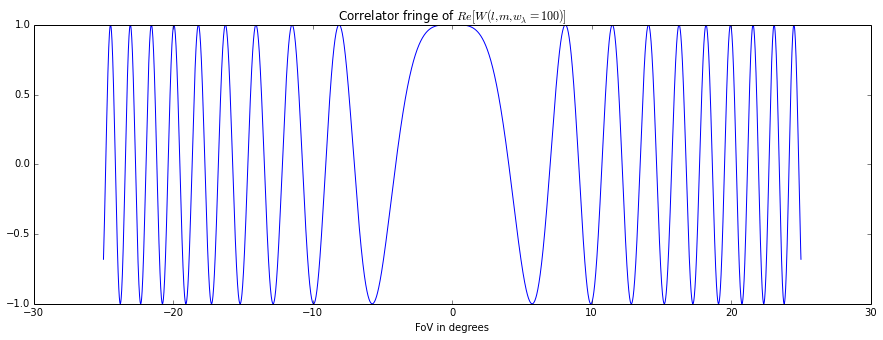
\includegraphics[width=\textwidth]{images/w_fringe_low_w.png}
      \caption{Low maximum w}
    \end{subfigure}  
    \begin{subfigure}[b]{0.7\textwidth}
      \centering
      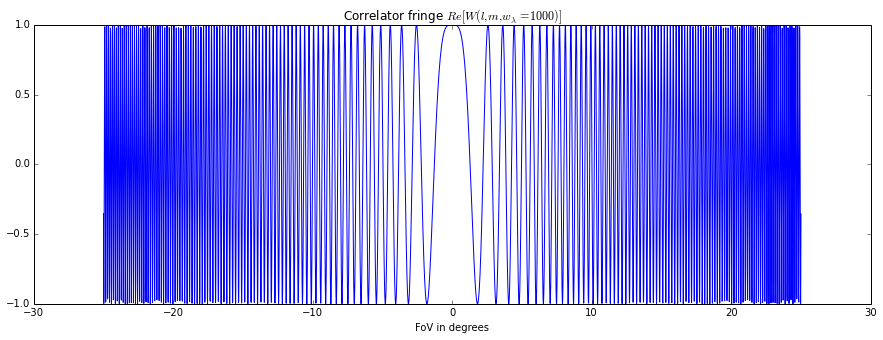
\includegraphics[width=\textwidth]{images/w_fringe_high_w.png}
      \caption{Higher maximum w}
    \end{subfigure}
    \caption[w fringe in one dimension]{Here the real part of the w phase term is plotted. It is clearly visible that the fringe is not scaled evenly over the field of view.
	       Instead the oscillations increase in frequency at the edge of the field of view, and has to be sampled in the image space at a rate that
	       satisfies the Nyquest sampling criteria. As expected for larger values of w (longer baselines) the frequency of the fringe osculations is
	       also increased.}
    \label{fig_w_fringes}
  \end{mdframed}
\end{figure}

By decreasing the field of view of each of the synthesized facets, it is ensured that the phase screen do not oscillate nearly as frequently as with a regular w-projection approach,
and decreases the required filter support size. Additionally the $\mathfrak{w}_w$ term can be separated into two functions of $l$ and $m$. If a small angle 
approximation ($\sqrt{1+x}\approx1+\frac{x}{2}$) to $\mathfrak{w}_w(l,m)$ with respect to a facet centre is used, the following separable relation is obtained:
\begin{equation}
   \mathfrak{w}_w(l,m) = e^{-2{\pi}iw[(l_i^2-l^2)/2]}e^{2{\pi}iw[(m_i^2-m^2)/2]}
\end{equation}

Assuming the normal anti-aliasing gridding function is separable as well this becomes:
\begin{equation}
   \begin{split}
   \mathcal{F}[\phi](l,m)\mathfrak{W}(l,m,w) &= \mathcal{F}[\phi](l)\mathcal{F}[\phi](m)e^{-2{\pi}iw[(l^2)/2]}e^{-2{\pi}iw[(m^2)/2]}\\
                             &= k(l)k(m)\\
                             &= k(l,m)\\
                             &\rightleftharpoons^\mathcal{F} K(u,v)\\
                             &=K(u)K(v)\\
   \end{split}
\end{equation}

This observation above decreases the memory requirements considerably, though the gridding time is slightly increased since two filter positions have to be looked up
and an additional complex multiplication is necessary during gridding. Note that the memory required to store filter is given by 
$N_{\text{planes}}\times[W_{sup} + (W_{sup} - 1)\times(m_{\text{oversampled}} - 1)]\times\mathbb{C}$. This is 
a $[W_{sup} + (W_{sup} - 1)\times(m_{\text{oversampled}} - 1)]$ reduction in memory consumption. This opens up the possibility of increasing $N_{\text{planes}}$ as well
as the oversampling rate. The accuracy of this small angle approximation is discussed in the next section.

To conclude this section we note that the sampling step size in the image domain (where the combination of $\mathfrak{w}_w\mathcal{F}[\phi]$ is sampled) is again given
by the Nyquest relation. Sample phase screens that include a simple $\sinc$ anti-aliasing filter are plotted in Figure~\ref{fig_phase_screen}.
\begin{equation}
 \begin{split}
  \Delta^l_{\text{convolution step}}&=\frac{1}{2N_{\text{sup}}\frac{\Delta{u}}{m_{\text{oversample}}}}\\
  \Delta^m_{\text{convolution step}}&=\frac{1}{2N_{\text{sup}}\frac{\Delta{v}}{m_{\text{oversample}}}}\\
 \end{split}
\end{equation}

\begin{figure}[h]
  \begin{mdframed}
    \centering
    \begin{subfigure}[b]{0.33\textwidth}
      \centering
      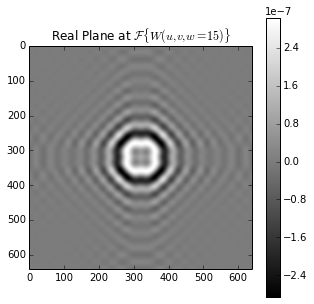
\includegraphics[width=\textwidth]{images/real_plane.png}
      \caption{}
    \end{subfigure}  
    \begin{subfigure}[b]{0.33\textwidth}
      \centering
      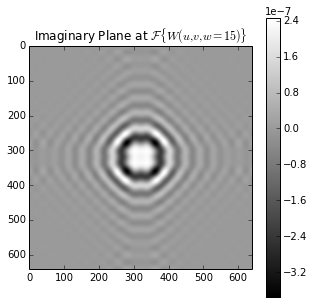
\includegraphics[width=\textwidth]{images/imag_plane.png}
      \caption{}
    \end{subfigure}
    \caption[Sample w phase screens]{Here the real (a) and imaginary (b) parts of the $\mathfrak{w}_w$ phase screens are plotted. 
	    In this plot $w_{\text{max}}/\lambda_{\text{min}} = 2000.000$. There are 32 planes between $w=0$ and the maximum.
	    The phase screen is simulated for a $5.1^\circ$ square image, with its half support size at 15 cells and $m_{\text{oversample}}=20$.
	    Here only a plane near the centre of the w range is plotted. Some aliasing effects are noticeable due to under sampling (due to memory
	    constraints).}
    \label{fig_phase_screen}
  \end{mdframed}
\end{figure}
\section{Error estimations}
Several methods of creating copanar facets have been discussed in the previous section. We give comparative plots in Figure~\ref{fig_error} where each of the methods is compared to
a traditional w-projection approach.
\begin{figure}[h]
  \begin{mdframed}
    \centering
    \begin{subfigure}[b]{0.7\textwidth}
      \centering
      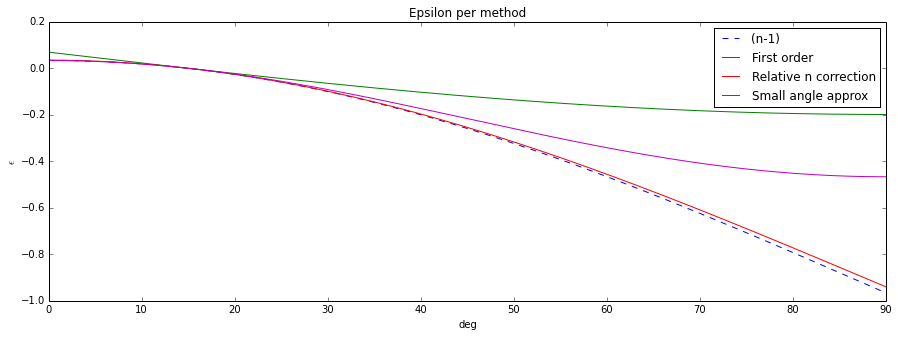
\includegraphics[width=\textwidth]{images/coplanar_error.png}
      \caption{}
    \end{subfigure}  
    \begin{subfigure}[b]{0.7\textwidth}
      \centering
      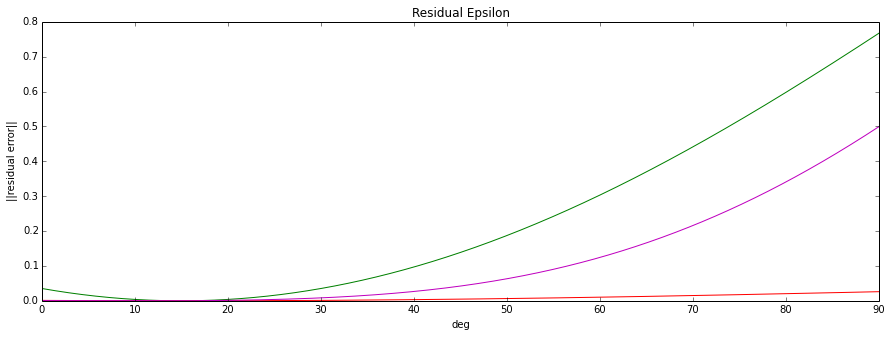
\includegraphics[width=\textwidth]{images/coplanar_error_residuals.png}
      \caption{}
    \end{subfigure}
    \caption[Coplanar faceting error]{In these two plots the phase error introduced by the orthogonal projection is plotted; the dashed line is a plot of $n-1$ as
    would be convolved into the image by classic w-projection; a full w-projection approach is assumed to be the most accurate way of dealing with the orthogonal projection geometry.
    In green we show the deviation between a first order Taylor approximation and w-projection\cite{aipsfaceting}. Then we show the small angle w-projection
    suggested above in magenta; it clearly performs significantly better than the first order approximation, only breaking down tens of degrees from the phase centre. Lastly we also
    plotted the improved facet-centre-relative w-kernel approximation to $\epsilon$ that Cyril\cite{tassefaceting} suggested as an improvement on the work of 
    Kogan and Greisen \cite{aipsfaceting} in red. Cyril's polynomial approach \cite{tassefaceting} performs even better than the latter. The error between w-projection and the three
    approaches is plotted in (b).}
    \label{fig_error}
  \end{mdframed}
\end{figure}

\section{Revisiting the direction-dependent effects}
Traditional calibration pipelines assumes that the same ``apparent sky'' is sampled by all antennae, and attempts to solve only the unknown direction-independent gain terms.
This process is known as \textit{self-calibration}. Furthermore some packages like the CASA framework consider directional dependent terms as simple effects 
that do not vary in time and is identical per antenna. The addition of directional dependencies within the all-sky integral, primarily those caused by the 
ionosphere and modulation effects by the primary beam, violates this premis. 

The self-calibration process relies on a knowing some aspects of the sky and can include one or more well-described sources. The directional
independent and directional dependent terms can be solved for by a fitting the predicted model visibilities to the observed 
data \cite{noordam2010meqtrees}. Only adjusting the gains based on directional-independent effects cannot remove the complex 
polarization effects caused by the primary beam, nor can it solve for unknown slow-varying directional dependent gain terms. If we, for 
the moment, only consider the known polarization effects of the antenna beam (which can be modeleled or measured using holography) it 
becomes clear that some sources will be more resolved than others for the same amount of observation time, 
depending on their position in the sky. In practice, the beam pattern is also anisotropic; one possible cause can be 
the struts above a prime-focus antenna. If the antennae are placed on alt-azumuth mounts the sky rotates with respect 
to this anisotropic beam pattern over the course of an observation. This results in sources that is only partially 
resolved everywhere other than well-within the primary beam. The correction of this effect alone is not a trivial undertaking - 
as the reader may suspect one possible solution is to attempt to ``invert'' the directional dependent effects on the visibility 
inside the convolution integral of the RIME.

Since these effects vary with both direction and time, removing them is a tricky proposition; at every timestep only a 
handful of points from these convolving functions are sampled! More recently several solutions to solve for slow-varying 
directional-dependent effects using self-calibration and removing known effects through calibration have been proposed. 
These include solving direction dependent effects through the method of differential gains, peeling and A-projection. Peeling 
involves iteratively removing the effects from the brightest sources through direct fourier approaches, while differential 
gains simultaniously solves for the gain effects from bright and faint sources \cite{2011A&A...527A.107S,2011A&A...527A.108S}. 
When dealing with known (or modeled) directional-dependent effects the A-projection algorithm \cite{bhatnagar2008correcting} has 
proven very successful in removing the polarization effects contributed (predominantly) by the primary beam for the 
LOFAR array (see figure~\ref{fig_aprojection_lofar}). Refer to the LOFAR imager implementation by Tasse et 
al. \cite{tasse2013applying} for a full mathematical treatment of the algorithm.

\begin{figure}[h!]
 \centering
 \begin{subfigure}[b]{0.35\textwidth}
  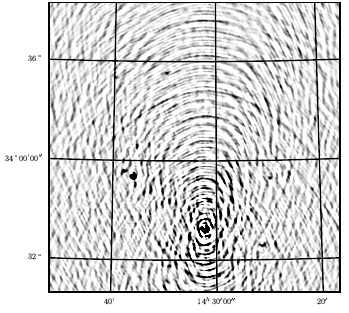
\includegraphics[width=\textwidth]{images/lofar_no_dd.png}
  \caption{Cleaned w-projected image}
 \end{subfigure}
 \begin{subfigure}[b]{0.35\textwidth}
  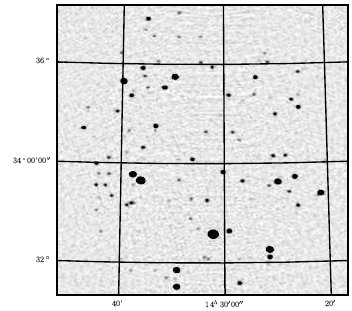
\includegraphics[width=\textwidth]{images/lofar_dd.png}
  \caption{Cleaned aw-projected image}
 \end{subfigure}
 \caption[A-projection results on LOFAR]{Figures (a) and (b) shows the result of correcting for the complex polarization leakage patterns
 introduced by the LOFAR individual element beams and phased-array stations}
 \label{fig_aprojection_lofar}
\end{figure}

In A-projection the ``union-form'' of the RIME stated before can be rewritten in terms of 16-element Muler matricies, for which first-order 
inverses can be computed. Provided that the 16 element terms vary slowly over the sky the inverses can be sampled at a limited number
of support points (far fewer than the w term stated previously) and can be convolved as part of the inversion step. A-projection does 
however require a significant amount of memory and time to precompute the 16 baseline-dependent (due to individual antenna pointing error) 
convolutions per processed visibility. As the number of baselines grow as the square of the number of antennae in this approach fast 
becomes prohiatively expensive \cite{tasse2013applying}.

An alternative strategy that can prove useful is to consider an amended faceting approach\footnote{Suggested by Cyril Tasse and Oleg Smirnov}. Here the 
direction-dependent effects are assumed to stay constant over a small area of the sky (centred at some $l_i,m_i$) and the Jones 
matrices may simply be inverted and applied as part of the part of the resampling process:
\begin{equation*}
 \begin{split}
 B_{\text{corrected,dirty}} &= \mathcal{F}^{-1}(D_p^{-1}(l_i,m_i,t,\nu)V_{\text{obs}}(u,v,t,\nu)D_q^{H^{-1}}(l_i,m_i,t,\nu))\\
			    &= \mathcal{F}^{-1}(D_p^{-1}(l_i,m_i,t,\nu)V_{\text{obs}}(u,v,t,\nu)D_q^{{-1}^H}(l_i,m_i,t,\nu))\\
 \end{split}
\end{equation*}

This approach has the additional advantage of being arbitrarily accurate: as the facet image size is decreased the inversion step
becomes a per-pixel corrected direct Fourier inversion. This makes this approach a viable alternative to A-projection. However, 
it must be stressed that the computation cost of both inversion and prediction steps rises sharply when creating polarization-corrected 
images with either approach: all four correlations must be gridded in stead of taking either only the parallel or cross-hand terms into 
account when doing traditional imaging. This effectively means that the number of floating point operations required by resampling 
effectively quadruples (the work in the inner most loop is four times more) without considering the additional conjugates taken and 
matrix multiplications for each observed visibility. Using this approach the additional storage required to store the 2x2 Jones 
matrices grows approximately as:
\begin{equation*}
 N_{\text{Jones}} \approx N_{\text{sources}}N_{\text{integration steps}}N_{\text{channels}}\sqrt{N_{\text{Baselines}}}
\end{equation*}

\section{Computational considerations}
We now draw a comparison of the computational complexities of the methods discussed here. Much of this discussion is taken from the detailed analysis of 
Yashar \& Kemball \cite{yashar2009tdp}.
The data\footnote{There are additional terms such as tapering weights, flags and metadata to consider, but these are ignored for now} rates produced by interferometers is roughly given as:
\begin{equation}
 r_\text{datarate} \approx \frac{1}{1024^4\tau_{\text{integration}}}N_{\text{baselines}}N_{\text{channels}}N_{\text{bands (spw)}}N_{\text{corr}}\text{sizeof}(\mathbb{C})\text{ (TiB/s)}
\end{equation}
where $\tau_{\text{integration}}$ is the correlator integration time, which depends on the effective resolution of the instrument and the rotation speed of the earth.
The maximum integration time must be short enough to ensure sources don't move more than the angular resolution of the telescope:
\begin{equation}
 \tau_{\text{integration}}^{-1} = Q_t\frac{|\vec{b}_{\text{max}}|}{D_{\text{antenna}}}\omega_\text{earth},\text{ where } \omega_\text{earth}\approx 7.29\times10^{-5}\text{rad}/\text{sec}_\text{Mean sidereal}
\end{equation}
Observing a bandlimited range of frequencies causes smeering in the image. Although a good signal to noise ratio depends on observing a large band of frequencies the smeering is only limited
by keeping bandwidth, $\Delta\nu$, of each channel narrow, centred at $\nu_i$. To compensate for the associated decrease in the signal to noise ratio of the observation many adjacent channels may be integrated if 
sources of continuum emission are being observed\footnote{We assume the intensity distribution of these sources do not vary significantly with frequency. This is in fact not true for wider bands; here 
it may be necessary to account for the drop in emission intensity, especially when deconvolving (using a Multifrequency approach, see for instance Conway and Sault \cite[Lecture 21]{taylor1999synthesis})}. In addition 
multiple channel bands (spectral windows) may be observed simultaniously. For continuum imaging the number of channels required is at minimum\footnote{It should 
be stressed that this number only limits the smeering in images. The actual number of channels used also depends on the science being done; spectral line imaging is just one instance where many more 
densely-packed channels may be required.}:
\begin{equation}
 N_{\text{channels}} = Q_c\frac{|\vec{b}_{\text{max}}|}{D_{\text{antenna}}}\frac{\Delta{\nu}}{\nu_i}
\end{equation}

Both $Q_t$ and $Q_c$ are quality factors.

Next we use slightly different equations for $N_\text{planes}$ and $N_\text{facets}$, in order to at least sample $n$ at the Nyquest rate in 3D imaging, W-projection (and W-stacking) and facet imaging. 
These equations assume only the primary beam is being imaged at the full effective resolution of the array (see e.g. Perley \cite[Lecture 19]{taylor1999synthesis}) for details on the derivation). 
Yashar \& Kemball \cite{yashar2009tdp} also use a different relation for the support of the convolution filters for W-projection.
\begin{equation}
 \begin{split}
  N_\text{planes} &\approx \frac{\lambda_{\text{max}}|\vec{b}_{\text{max}}|}{\xi D_{\text{antenna}}}\\
  N_\text{facets}^2 &\approx \left(\frac{2\lambda_{\text{max}}|\vec{b}_{\text{max}}|}{\xi D_{\text{antenna}}}\right)^2\\
  w_\text{sup}^2 &\approx \left(\frac{2\lambda_{\text{max}}|\vec{b}_{\text{max}}|}{D_{\text{antenna}}}\right)^2\\
 \end{split}
\end{equation}
Table~\ref{tbl_computational complexities} outlines the computational complexities for the backward synthesis step only. Some of these methods may have additional computational costs for prediction, deconvolution and reprojections.
\begin{table}[ht]
  \centering
  \begin{tabular}[c]{|p{7cm}|c|}
  \hline
  \textbf{Approach} & \textbf{Computational complexity (backwards step only)}\\
  \hline
  (Cubed) Direct Fourier Transform & $MN^3$\\
  \hline
  3D Imaging using FFT &$N_\text{planes}(M + MC^2 + 2N^2\log{N})$\\
  \hline
  Traditional non-coplanar faceting & $N_\text{facets}^2(M + MC^2 + 2N_f^2\log{N_f})$\\
  \hline
  W-projection & $Mw_\text{sup}^2+2N^2\log{N}$\\
  \hline
  W-stacking & $MC^2 + N_\text{planes}(2N^2\log{N} + N^2)$\\
  \hline
  \end{tabular}
  \caption[]{}
  \label{tbl_computational complexities}
\end{table}

The cubed Direct Fourier Transform is a per-voxel complex exponential and multiplication. The real sky lies on a unit sphere in the cube. The approach is prohibitively expensive both
in terms of memory and computational complexity ($M$ scales as $N^2$), though arbitrarily accurate. 

The FFT-based 3D Imaging approach each plane has it's visibilities phase steared, then interpolated onto a grid and fourier transformed seperately using a 2D fourier transform \cite[Lecture 19]{taylor1999synthesis}. 
Alternatively if there are enough planes in the $n$ dimension the visibilties can be interpolated directly into a cube and a three-dimensional Fast Fourier Transform taken \cite{yashar2009tdp}. This approach also has prohibative memory
requirements.

A faceting approach requires that the set of visibilties are phase-steered and sampling coordinates transformed while gridding and a Fourier transform of each smaller field is taken. Each field hare approximately 
$N_f^2=\left(\frac{0.4|\vec{b}_\text{max}|}{D_\text{antenna}}\right)^2$ pixels for $\xi=0.2$.

W-projection becomes expensive with a large field of view, but can be faster than w-stacking for a small number of visibilities. Keeping many oversampled convolution kernel layers in memory is one drawback
of this method, unless a small-angle approximation can be applied to the kernels, or by limiting the support size of the convolution filters in the lower w-layers \cite{offringa2014wsclean}.

In W-stacking each visibility is gridded with the usual gridding convolution function $\phi$, but to different planes depending on w. Each plane is fourier transformed and 
multiplied by a complex phase screen. This approach works well for large sets of visibilities where the FFT costs per grid is negligible. The approach can be demanding in terms of memory depending
on the number of w-planes being gridded, and may require presorting and gridding only a subset of layers at a time, increasing disk access. The approach is faster than w-projection
for larger fields of view and at lower elevation angles. Offringa et al. also shows that w-snapshots are only faster than w-stacking for very large fields of view at lower elivation angles \cite{offringa2014wsclean}.

From the estimates above for number of projection planes and facets it is clear that w-stacking will outperform faceting if all the planes can be kept in memory and the gridding costs exceed fourier transformation costs. 
However, as already pointed out faceting has more moderate memory requirements than w-stacking and can furthermore be used as an approximate method for correcting Directional Dependent Effects.
\section{Review of previous literature}
The imaging pipeline has been investigated extensively in recent years. In particular the gridding operation has been parallelized multiple architectures including CPU \cite{offringa2014wsclean,golap2015mutithreading,obitfaceting}, 
GPU \cite{humphreys2011analysis,romein2012efficient,muscat2014high,edgar2010enabling}, as well as the CELL/B.E. processor \cite{varbanescu2008performance}. 

Both scatter- and gather-based GPU gridding algorithms have been investigated in the literature. In gridding scatter-based approaches lead to race conditions between
threads when updating grid cells, since multiple visibilties may be interpolated over the same grid cells. Edgar et al. \cite{edgar2010enabling} used a gather approach where 
threads would scan through a subset of visibilities and add those that contribute to a the grid point in question. Edgar et al. attains a 22x speedup compared to a CPU implemented pipeline.  

Humphreys and Cornwell \cite{humphreys2011analysis} benchmarked a scatter-based GPU w-projection gridder that assigns a thread per convolution filter tap and can grid multiple visibilities in parallel when there is no overlap
between the convolution regions. They report figures up to 3.5 Giga grid point additions per second (abbreviated as ``G'' is the number of grid point updates - $C^2$ updates per visibility record) on a Tesla C2070 compared to 
just over 1.5 G on a multicore Intel Xeon X5570 CPU architecture. 

Romein \cite{romein2012efficient} presents a novel scatter distribution strategy, where global memory accesses are limited by accumulating visibilities in register memory instead of atomically updating
each grid points for every visibility record. The locality of consecutive integration periods on the loci of each baseline is used to accumulate consecutive visibilities to great succcess. 
Muscat \cite{muscat2014high} uses this distribution strategy in a new imager called the \textit{Malta Imager}. He achieves gridding rates of around 55-60G when gridding 4 correlations. He also
shows that the main limiting factor in this distribution strategy is the time spent looking up convolution filter values and extends Romein's strategy by accumulating measurements that have a high probability
of being equal. When this ``compression'' mode is enabled he achieves gridding rates more than 250G. We will be using an adapted strategy based on Romein's distribution strategy in this thesis. The exact algorithmic details will be given in the design chapter.

The CPU-based parallel strategies are somewhat different to the GPU-based strategies. A simple data-parallel approach in spectral imaging consists of splitting the image cube up between threads as is done by Humphreys and Cornwell \cite{humphreys2011analysis} for
their CPU-based benchmark. A data-parallel approach for continuim imaging consists of keeping multiple copies of the uv grid and reducing the grids into one average
afterwards. This is not feasible when the uv grids become very large. Kumar Goulap \cite{golap2015mutithreading} investigates several CPU-based gather approaches applicable to w-projection and show that
this can achieve near-linear speedups (compared to a serial implementation). When doing faceting another lock-free data-parallel approach is to process each facet in parallel, ensuring lock-free accumulation
to each facet uv grid. Bill Cotton \cite{obitfaceting} achieved speedups up to 50\% using data-parallel approaches.